\chapter{Manifold and Fibre Bundle}
\label{chap:manifold}
\markboth{Manifold Foundations and Fibre Bundles}{Manifold Foundations and Fibre Bundles}

\begin{remark}[Positioning of This Chapter]\label{rem:manifold_chapter_positioning}
This chapter establishes the language of manifolds for the geometric analysis of periodic orbits. The core object of periodic mathematics is a closed curve in a state space; to determine rigorously whether an orbit is closed, to describe the geometric structure of periodic evolution, and to characterise the constraints that conservation laws impose on orbits, the language of manifolds is required.

Manifolds serve three core functions in this chapter:
\begin{enumerate}[label=(\arabic*)]
    \item \textbf{Criterion for the closure of an orbit}: a closed orbit is a closed curve on a manifold, and its closure is characterised by an element of finite order in the fundamental group (Definition \ref{def:closed_orbit_manifold}); the torus, as the quotient manifold $\mathbb{R}^d/\Lambda$, provides a global classification of closed orbits (Proposition \ref{prop:periodic_manifold_fundamental_group}).
    \item \textbf{Geometric stage of periodic evolution}: periodic evolution takes place on the state-space manifold; its instantaneous direction is described by the tangent space (Definition \ref{def:tangent_vector_derivation}), the constraints of conservation laws are described by the normal space (Definition \ref{def:normal_space}), and the parametrisation of phase is described by the angle space (Definition \ref{def:angle_space}).
    \item \textbf{Geometric realisation of conservation laws}: the level set of a conserved quantity is a submanifold (Theorem \ref{thm:regular_level_set}), orbits are constrained to lie on invariant submanifolds (Definition \ref{def:invariant_submanifold}), and the orbits of an integrable system lie on invariant tori (Definition \ref{def:invariant_torus}).
\end{enumerate}

\textbf{Guide to the seven themes of this chapter}: Translation --- the tangent vector as the infinitesimal generator of translation (Definition \ref{def:tangent_vector_derivation}), the orbits of a group action (Definition \ref{def:group_action_manifold}), the covering map $\mathbb{R} \to S^1$ (Theorem \ref{thm:covering_R_S1}); Scaling --- the scaling of the Riemannian metric (Definition \ref{def:riemannian_metric}), the orthogonal complement of the normal space (Definition \ref{def:normal_space}), the parametrisation of the moduli space (Definition \ref{def:moduli_space}); Rotation --- the $U(1)$ structure of the angle space (Definition \ref{def:angle_space}), the rotation of the invariant torus (Definition \ref{def:invariant_torus}), the spiralling of the stable/unstable manifolds (Definition \ref{def:stable_unstable_manifold}); Conservation --- the level set of a conserved quantity as a submanifold (Theorem \ref{thm:regular_level_set}), the energy surface (Definition \ref{def:energy_surface}), the constraints of the normal bundle (Proposition \ref{prop:normal_bundle_constraint}); Symmetry --- group actions and quotient manifolds (Definition \ref{def:quotient_manifold}); Closure --- closed orbits and the fundamental group (Definition \ref{def:closed_orbit_manifold}), the classification of the fundamental group of the torus (Proposition \ref{prop:periodic_manifold_fundamental_group}); Period --- the torus as the quotient manifold $\mathbb{R}^d/\Lambda$ (Proposition \ref{prop:torus_quotient}), periodic and quasi-periodic motion on an invariant torus (Proposition \ref{prop:invariant_torus_motion}).
\end{remark}

\begin{figure}[htbp]
\centering
\begin{tikzpicture}[
  font=\small,
  box/.style={draw, rounded corners, fill=blue!8, minimum width=2.4cm, minimum height=0.8cm, align=center},
  sub/.style={draw, rounded corners, fill=green!10, minimum width=2.2cm, minimum height=0.7cm, align=center, font=\footnotesize},
  arr/.style={->, thick, >=stealth}
]
  % First row: three classes of geometric object
  \node[box] (manifold) {topological/smooth manifold\\locally Euclidean space};
  \node[box, right=1.0cm of manifold] (bundle) {fibre bundle\\local trivialisation};
  \node[box, right=1.0cm of bundle] (riem) {Riemannian manifold\\metric structure};
  % Second row: core structures
  \node[sub, below=0.9cm of manifold] (tan) {tangent space/tangent bundle\\instantaneous direction};
  \node[sub, below=0.9cm of bundle] (cotan) {cotangent space/cotangent bundle\\differential 1-forms};
  \node[sub, below=0.9cm of riem] (norm) {normal space/normal bundle\\conservation constraints};
  % Third row: periodic objects
  \node[box, fill=orange!12, below=1.0cm of tan] (torus) {invariant torus $\mathbb{T}^n$\\periodic and quasi-periodic};
  \node[box, fill=orange!12, below=1.0cm of cotan] (phase) {phase space $T^*Q$\\symplectic structure};
  \node[box, fill=orange!12, below=1.0cm of norm] (orbit) {closed orbits\\classification by the fundamental group};
  % Arrows
  \draw[arr] (manifold) -- (bundle);
  \draw[arr] (bundle) -- (riem);
  \draw[arr] (manifold) -- (tan);
  \draw[arr] (bundle) -- (cotan);
  \draw[arr] (riem) -- (norm);
  \draw[arr] (tan) -- (torus);
  \draw[arr] (cotan) -- (phase);
  \draw[arr] (norm) -- (orbit);
\end{tikzpicture}
\caption{Overview of the structure of this chapter: starting from topological/smooth manifolds, passing through fibre bundles and Riemannian structure, and leading to the tangent, cotangent and normal bundles, which finally converge on the three periodic objects: the invariant torus, phase space and closed orbits.}
\label{fig:manifold_overview}
\end{figure}

\section{Topological and Smooth Manifolds}

\begin{definition}[Topological Manifold]\label{def:topological_manifold}
Let $M$ be a topological space. $M$ is called an $n$-dimensional \textbf{topological manifold} if it satisfies:
\begin{enumerate}[label=(\roman*)]
    \item \textbf{Hausdorff property}: for any $p \neq q \in M$ there exist open neighbourhoods $U \ni p$ and $V \ni q$ with $U \cap V = \emptyset$;
    \item \textbf{Second countability}: $M$ has a countable topological basis;
    \item \textbf{Local Euclidean property}: for any $p \in M$ there exist an open neighbourhood $U \ni p$ and a homeomorphism $\varphi: U \to \varphi(U) \subseteq \mathbb{R}^n$.
\end{enumerate}
$(U, \varphi)$ is called a \textbf{chart} of $M$ near $p$, and $\varphi(p) = (x^1(p), \dots, x^n(p))$ are called the \textbf{local coordinates} of $p$.
\end{definition}

\begin{figure}[htbp]
\centering
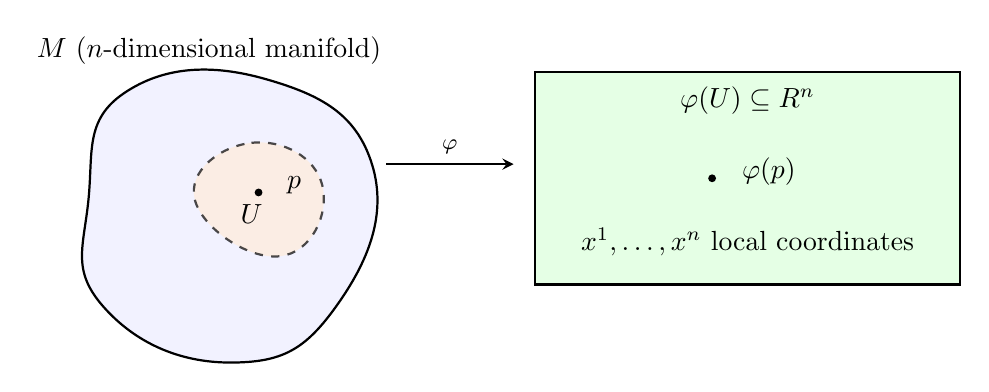
\begin{tikzpicture}[scale=0.9]

  \draw[thick, fill=blue!5] plot[smooth cycle, tension=0.8] coordinates {(-2,0.5) (-1.5,2) (0.5,2.2) (2,1) (1.5,-1) (0,-1.8) (-1.8,-1)};
  \node at (-0.3,2.6) {$M$ ($n$-dimensional manifold)};

  \draw[thick, dashed, fill=orange!15, opacity=0.7] plot[smooth cycle, tension=0.9] coordinates {(-0.5,0.5) (0.3,1.3) (1.3,0.7) (0.7,-0.3)};
  \node at (0.3,0.3) {$U$};
  \node[circle, fill, inner sep=1pt] at (0.4,0.6) {};
  \node at (0.9,0.7) {$p$};

  \draw[->, thick, >=stealth] (2.2,1) -- node[above, font=\footnotesize]{$\varphi$} (4.0,1);

  \draw[thick, fill=green!10] (4.3,-0.7) rectangle (10.3,2.3);

  \node at (7.3,1.9) {$\varphi(U)\subseteq\mathbb{R}^n$};
  \node[circle, fill, inner sep=1pt] at (6.8,0.8) {};
  \node at (7.6,0.9) {$\varphi(p)$};
  \node at (7.3,-0.1) {$x^1,\dots,x^n$ local coordinates};
\end{tikzpicture}
\caption{The local Euclidean property of a topological manifold: the neighbourhood $U$ of $p$ is homeomorphic, via the chart $\varphi$, to an open set in $\mathbb{R}^n$.}
\label{fig:topological_manifold_chart}
\end{figure}

\begin{example}[Basic Examples of Manifolds]\label{ex:manifold_examples}
\begin{enumerate}[label=(\roman*)]
    \item $\mathbb{R}^n$ itself is an $n$-dimensional topological manifold (take the identity map as a global chart).
    \item The circle $S^1 = \{(x,y) \in \mathbb{R}^2 : x^2 + y^2 = 1\}$ is a $1$-dimensional topological manifold. One may take two charts: $U_1 = S^1 \setminus \{(1,0)\}$, $\varphi_1(\cos\theta, \sin\theta) = \theta \in (0, 2\pi)$; $U_2 = S^1 \setminus \{(-1,0)\}$, $\varphi_2(\cos\theta, \sin\theta) = \theta \in (-\pi, \pi)$.
    \item The $n$-dimensional torus $\mathbb{T}^n = S^1 \times \cdots \times S^1$ is an $n$-dimensional topological manifold.
    \item The $n$-dimensional sphere $S^n = \{\mathbf{x} \in \mathbb{R}^{n+1} : \|\mathbf{x}\| = 1\}$ is an $n$-dimensional topological manifold.
\end{enumerate}
\end{example}

\begin{definition}[Smooth Manifold]\label{def:smooth_manifold}
Let $M$ be a topological manifold. A \textbf{smooth atlas} on $M$ is a family of charts
\[
\begin{aligned}
&\{(U_\alpha, \varphi_\alpha)\}_{\alpha \in A}
\end{aligned}
\]
satisfying:
\begin{enumerate}[label=(\roman*)]
    \item $\{U_\alpha\}_{\alpha \in A}$ covers $M$;
    \item for any $\alpha, \beta$, if $U_\alpha \cap U_\beta \neq \emptyset$, then the transition map
    \[
    \varphi_\beta \circ \varphi_\alpha^{-1}: \varphi_\alpha(U_\alpha \cap U_\beta) \to \varphi_\beta(U_\alpha \cap U_\beta)
    \]
    is a $C^\infty$ smooth map.
\end{enumerate}
A topological manifold equipped with a maximal smooth atlas is called a \textbf{smooth manifold}.
\end{definition}

\begin{figure}[htbp]
\centering
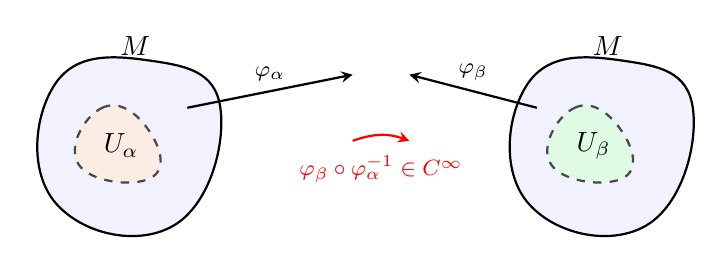
\begin{tikzpicture}[scale=0.6]

  \draw[thick, fill=blue!5] plot[smooth cycle, tension=0.8] coordinates {(-2,-0.5) (-2,2) (0,2.5) (1.5,1.5) (0.5,-1)};
  \draw[thick, dashed, fill=orange!15, opacity=0.7] plot[smooth cycle, tension=0.9] coordinates {(-1.5,0.3) (-1,1.5) (0,1) (0,0)};
  \node at (-0.6,0.7) {$U_\alpha$};
  \node at (-0.3,2.8) {$M$};

  \draw[thick, fill=blue!5] plot[smooth cycle, tension=0.8] coordinates {(8,-0.5) (8,2) (10,2.5) (11.5,1.5) (10.5,-1)};
  \draw[thick, dashed, fill=green!15, opacity=0.7] plot[smooth cycle, tension=0.9] coordinates {(8.5,0.3) (9,1.5) (10,1) (10,0)};
  \node at (9.4,0.7) {$U_\beta$};
  \node at (9.7,2.8) {$M$};

  \draw[->, thick, >=stealth] (0.8,1.5) -- node[above, font=\footnotesize]{$\varphi_\alpha$} (4.3,2.2);

  \draw[->, thick, >=stealth] (8.2,1.5) -- node[above, font=\footnotesize]{$\varphi_\beta$} (5.5,2.2);

  \draw[->, thick, >=stealth, red] (4.3,0.8) to[bend left=20] (5.5,0.8);
  \node[red, font=\footnotesize] at (4.9,0.2) {$\varphi_\beta\circ\varphi_\alpha^{-1}\in C^\infty$};

\end{tikzpicture}
\caption{Transition maps of a smooth manifold: on the overlap of two charts the transition map $\varphi_\beta\circ\varphi_\alpha^{-1}$ is smoothly compatible.}
\label{fig:smooth_manifold_charts}
\end{figure}

\begin{definition}[Smooth Functions and Smooth Maps]\label{def:smooth_function_map}
Let $M$ be a smooth manifold.
\begin{enumerate}[label=(\roman*)]
    \item A function $f: M \to \mathbb{R}$ is called \textbf{smooth} if for every chart $(U, \varphi)$ the map $f \circ \varphi^{-1}$ is $C^\infty$. The set of all smooth functions on $M$ is denoted $C^\infty(M)$.
    \item A map $F: M \to N$ is called \textbf{smooth} if for every $p \in M$ the map $\psi \circ F \circ \varphi^{-1}$ is $C^\infty$.
    \item If $F$ is a bijection and both $F$ and $F^{-1}$ are smooth, then $F$ is called a \textbf{diffeomorphism}.
\end{enumerate}
\end{definition}

\section{Tangent Space and Tangent Bundle}

\begin{definition}[Tangent Vector---Derivation Definition]\label{def:tangent_vector_derivation}
Let $M$ be a smooth manifold and $p \in M$. A \textbf{tangent vector} at $p$ is a linear map $v: C^\infty(M) \to \mathbb{R}$ satisfying the Leibniz rule:
\[
v(fg) = v(f) g(p) + f(p) v(g), \qquad \forall f, g \in C^\infty(M).
\]
The set of all tangent vectors at $p$ is denoted $T_pM$ and is called the tangent space.
\end{definition}

\begin{proposition}[Dimension and Coordinate Basis of the Tangent Space]\label{prop:tangent_space_basis}
Let $M$ be an $n$-dimensional smooth manifold, $p \in M$, and let $(U, \varphi = (x^1, \dots, x^n))$ be a chart. Then $T_pM$ has dimension $n$, and a basis is given by $\left. \frac{\partial}{\partial x^1} \right|_p, \dots, \left. \frac{\partial}{\partial x^n} \right|_p$.
\end{proposition}

\begin{proof}
\textbf{Step 1 (verifying that $\left. \frac{\partial}{\partial x^i} \right|_p$ is a tangent vector)}. Linearity is given by the linearity of partial derivatives; the Leibniz rule is given by the product rule for partial derivatives.

\textbf{Step 2 (linear independence)}. Suppose that $\sum_i a^i \left. \frac{\partial}{\partial x^i} \right|_p = 0$. Taking the coordinate function $x^j$, we obtain $0 = \sum_i a^i \frac{\partial x^j}{\partial x^i} = a^j$.

\textbf{Step 3 (spanning)}. For any $v$ and $f$, expand $f \circ \varphi^{-1}$ to first order by Taylor's theorem at $p$; applying $v$ then gives $v(f) = \sum_i v(x^i) \frac{\partial f}{\partial x^i}(p)$. Hence $\{ \partial_i|_p \}$ spans $T_pM$.
\end{proof}

\begin{figure}[htbp]
\centering
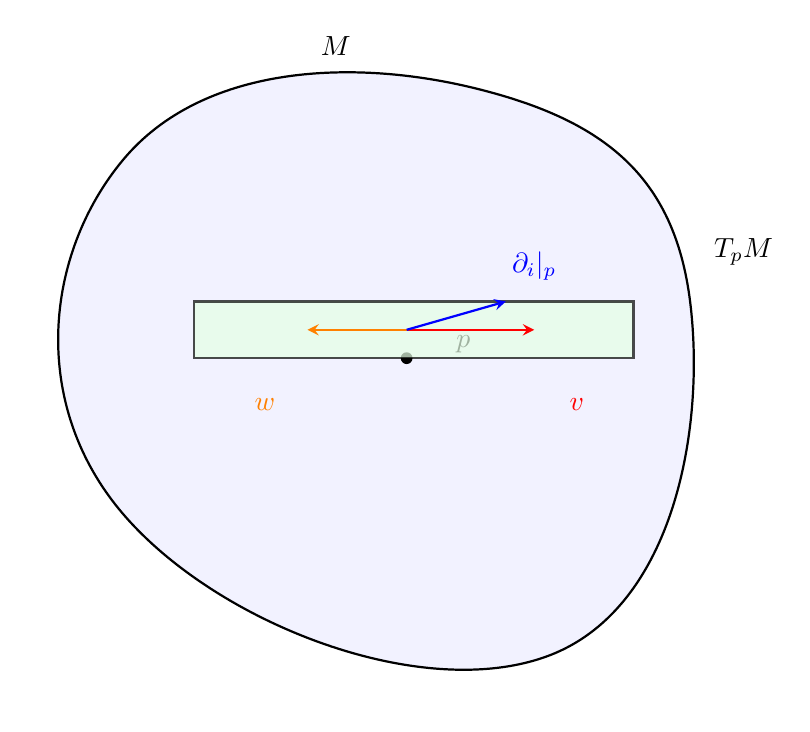
\begin{tikzpicture}[scale=1.8]

  \draw[thick, fill=blue!5] plot[smooth cycle, tension=0.8] coordinates {(-2,-0.5) (-2,2) (0.5,2.5) (2,1) (1,-1.5)};
  \node at (-0.5,2.8) {$M$};

  \node[circle, fill, inner sep=1.5pt] (p) at (0,0.6) {};
  \node at (0.4,0.7) {$p$};

  \draw[thick, fill=green!10, opacity=0.7] (-1.5,0.6) -- (1.6,0.6) -- (1.6,1.0) -- (-1.5,1.0) -- cycle;
  \node[xshift=0.5cm] at (2.1,1.35) {$T_pM$};

  \draw[->, thick, red, >=stealth] (0,0.8) -- (0.9,0.8);
  \node[red, yshift=-0.5cm] at (1.2,0.55) {$v$};
  \draw[->, thick, orange, >=stealth] (0,0.8) -- (-0.7,0.8);
  \node[orange, yshift=-0.5cm] at (-1.0,0.55) {$w$};

  \draw[->, thick, blue, >=stealth] (0,0.8) -- (0.7,1.0);
  \node[blue] at (0.9,1.25) {$\partial_i|_p$};
\end{tikzpicture}
\caption{The tangent space $T_pM$ is the linearisation of $M$ at $p$: a tangent vector is an infinitesimal displacement tangential to the manifold.}
\label{fig:tangent_space}
\end{figure}

\begin{definition}[Tangent Vector---Curve Equivalence Class Definition]\label{def:tangent_vector_curve}
Let $M$ be a smooth manifold and $p \in M$. Let $\mathcal{C}_p$ denote the set of smooth curves through $p$. Define an equivalence relation on $\mathcal{C}_p$ by $\gamma_1 \sim \gamma_2$ if and only if $\frac{d}{dt}(\varphi \circ \gamma_1)(0) = \frac{d}{dt}(\varphi \circ \gamma_2)(0)$. The equivalence class $[\gamma]$ is called a tangent vector.
\end{definition}

\begin{lemma}[Equivalence of the Two Definitions of Tangent Vectors]\label{lem:tangent_vector_equivalence}
The derivation definition (Definition \ref{def:tangent_vector_derivation}) and the curve equivalence class definition (Definition \ref{def:tangent_vector_curve}) give the same tangent space. The correspondence is:
\[
[\gamma] \mapsto v_{[\gamma]}, \qquad v_{[\gamma]}(f) = \left. \frac{d}{dt} \right|_{t=0} f(\gamma(t)).
\]
\end{lemma}

\begin{figure}[htbp]
\centering
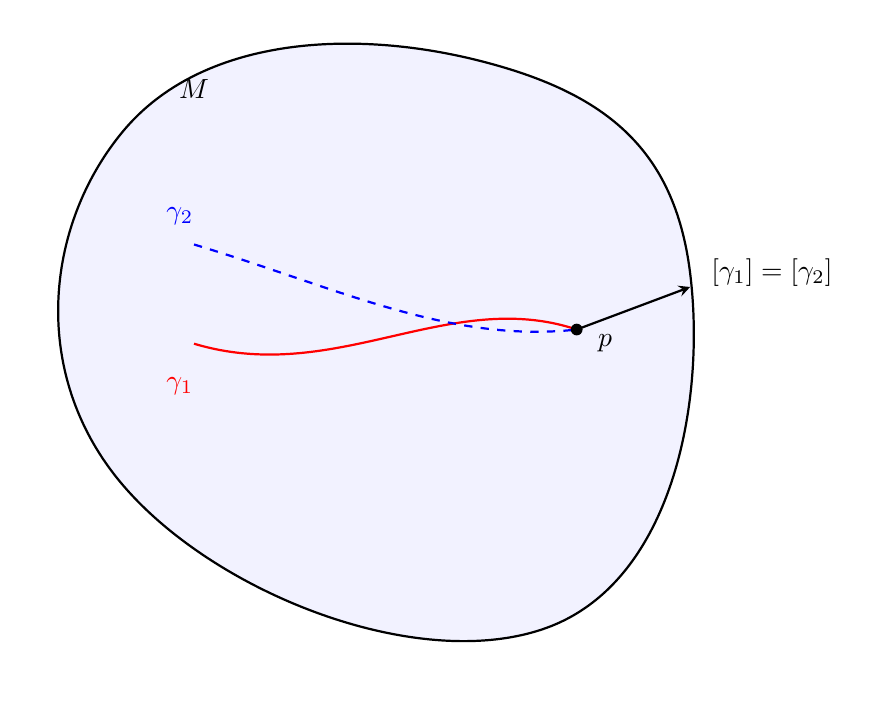
\begin{tikzpicture}[scale=1.8]

  \draw[thick, fill=blue!5] plot[smooth cycle, tension=0.8] coordinates {(-2,-0.5) (-2,2) (0.5,2.5) (2,1) (1,-1.5)};
  \node at (-1.5,2.3) {$M$};

  \draw[thick, red] (-1.5,0.5) .. controls (-0.5,0.2) and (0.3,0.9) .. (1.2,0.6);
  \draw[thick, blue, dashed] (-1.5,1.2) .. controls (-0.5,0.9) and (0.3,0.5) .. (1.2,0.6);
  \node[red] at (-1.6,0.2) {$\gamma_1$};
  \node[blue] at (-1.6,1.4) {$\gamma_2$};
  \node[circle, fill, inner sep=1.5pt] at (1.2,0.6) {};
  \node at (1.4,0.5) {$p$};

  \draw[->, thick, black, >=stealth] (1.2,0.6) -- (2.0,0.9);
  \node[xshift=0.5cm] at (2.3,1.0) {$[\gamma_1]=[\gamma_2]$};
\end{tikzpicture}
\caption{The two definitions of a tangent vector: curves through the same point with the same velocity at that point belong to the same equivalence class and correspond to the same tangent vector.}
\label{fig:tangent_vector_equivalence}
\end{figure}

\begin{proof}
\textbf{Step 1 (well-definedness)}. If $\gamma_1 \sim \gamma_2$, then for any $f$,
\[
\left. \frac{d}{dt} \right|_{t=0} f(\gamma_1(t)) = df_p\left( \frac{d}{dt}(\varphi\circ\gamma_1)(0) \right) = df_p\left( \frac{d}{dt}(\varphi\circ\gamma_2)(0) \right) = \left. \frac{d}{dt} \right|_{t=0} f(\gamma_2(t)).
\]

\textbf{Step 2 ($v_{[\gamma]}$ is a derivation)}. Linearity is given by the linearity of the derivative. The Leibniz rule is given by the product rule.

\textbf{Step 3 (surjectivity)}. Given a derivation $v = \sum_i a^i \frac{\partial}{\partial x^i}$, take $\gamma(t) = \varphi^{-1}(\varphi(p) + t(a^1, \dots, a^n))$; then $v_{[\gamma]} = v$.

\textbf{Step 4 (injectivity)}. If $v_{[\gamma_1]} = v_{[\gamma_2]}$, then for the coordinate functions $x^i$, $\frac{d}{dt}(\varphi \circ \gamma_1)^i(0) = \frac{d}{dt}(\varphi \circ \gamma_2)^i(0)$, hence $\gamma_1 \sim \gamma_2$.
\end{proof}

\begin{definition}[Tangent Bundle]\label{def:tangent_bundle}
The \textbf{tangent bundle} of $M$ is defined as $TM := \bigsqcup_{p \in M} T_pM$, equipped with the projection $\pi: TM \to M$. A \textbf{vector field} on $M$ is a smooth section of the tangent bundle.
\end{definition}

\begin{proposition}[Manifold Structure of the Tangent Bundle]\label{prop:tangent_bundle_manifold}
The tangent bundle $TM$ is a $2n$-dimensional smooth manifold.
\end{proposition}

\begin{proof}
Let $(U, \varphi)$ be a chart of $M$.
Define the corresponding chart $(\pi^{-1}(U), \tilde{\varphi})$ on $TM$,
where
$\tilde{\varphi}(p, v) = (x^1(p), \dots, x^n(p), v^1, \dots, v^n)$.
The smoothness of the transition map follows from
\[
\begin{aligned}
  \tilde{\varphi}_\beta \circ \tilde{\varphi}_\alpha^{-1}(x, v)
  = \bigl(y(x), \sum_i \tfrac{\partial y}{\partial x^i} v^i\bigr)
\end{aligned}
\]
where $y = \varphi_\beta \circ \varphi_\alpha^{-1} \in C^\infty$,
whose partial derivatives are also $C^\infty$.
\end{proof}

\begin{figure}[htbp]
\centering
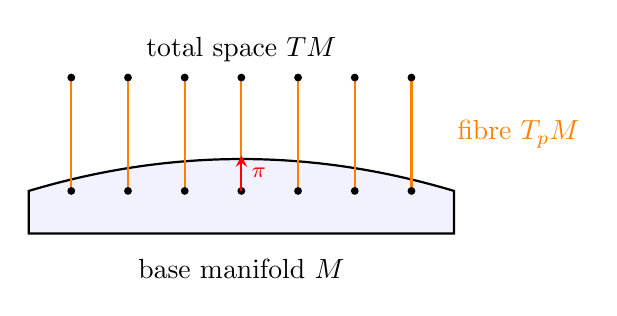
\begin{tikzpicture}[scale=0.9]

  \draw[thick, fill=blue!5] (-3,-2) -- (3,-2) -- (3,-1.4) .. controls (1,-0.8) and (-1,-0.8) .. (-3,-1.4) -- cycle;
  \node at (0,-2.5) {base manifold $M$};

  \foreach \x in {-2.4,-1.6,-0.8,0,0.8,1.6,2.4} {
    \draw[thick, orange] (\x,-1.4) -- (\x,0.2);
    \node[circle, fill, inner sep=1pt] at (\x,-1.4) {};
    \node[circle, fill, inner sep=1pt] at (\x,0.2) {};
  }
  \node[orange, xshift=1cm] at (2.8,-0.6) {fibre $T_pM$};
  \node at (0,0.6) {total space $TM$};

  \draw[->, thick, >=stealth, red] (0,-1.4) -- node[right, font=\footnotesize]{$\pi$} (0,-0.9);
\end{tikzpicture}
\caption{The tangent bundle $TM$: with the base manifold $M$ as base, the tangent space $T_pM$ hangs above each point $p$ as the fibre, and the projection $\pi$ maps $(p,v)$ back to $p$.}
\label{fig:tangent_bundle}
\end{figure}

\section{Cotangent Space and Cotangent Bundle}

\begin{definition}[Cotangent Space and Differential]\label{def:cotangent_space}
$T_p^*M := (T_pM)^*$ is called the \textbf{cotangent space}. For $f \in C^\infty(M)$, $df_p(v) := v(f)$ is called the \textbf{differential} of $f$ at $p$.
\end{definition}

\begin{proposition}[Coordinate Basis of the Cotangent Space]\label{prop:cotangent_basis}
Let $(U, \varphi = (x^1, \dots, x^n))$ be a chart. Then a basis of $T_p^*M$ is $dx^1|_p, \dots, dx^n|_p$, satisfying $dx^i|_p(\frac{\partial}{\partial x^j}|_p) = \delta_j^i$.
\end{proposition}

\begin{proof}
By Proposition \ref{prop:tangent_space_basis}, $\{\frac{\partial}{\partial x^i}\}$ is a basis of $T_pM$. By the dual basis theorem of linear algebra, there exists a unique dual basis $\{\omega^i\}$ satisfying $\omega^i(\frac{\partial}{\partial x^j}) = \delta_j^i$. Let us verify that $\omega^i = dx^i$: for any $v = \sum_j v^j \frac{\partial}{\partial x^j}$,
\[
dx^i(v) = v(x^i) = \sum_j v^j \frac{\partial x^i}{\partial x^j} = v^i = \omega^i(v).
\]
Hence $dx^i$ is precisely the dual basis.
\end{proof}

\begin{figure}[htbp]
\centering
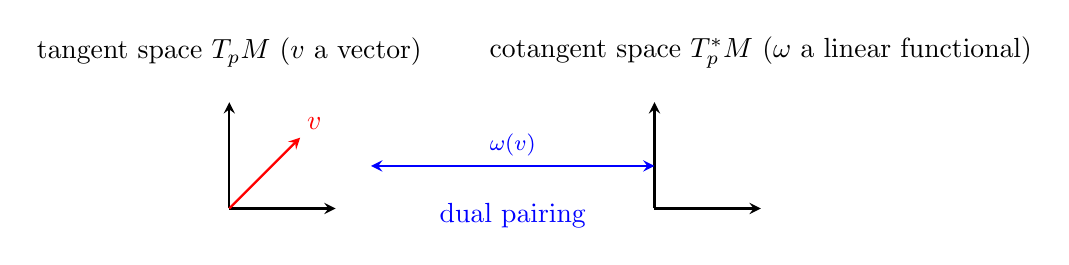
\begin{tikzpicture}[scale=0.9]

  \node at (0,2.2) {tangent space $T_pM$ ($v$ a vector)};
  \draw[thick, ->, >=stealth] (0,0) -- (1.5,0);
  \draw[thick, ->, >=stealth] (0,0) -- (0,1.5);
  \draw[->, thick, red, >=stealth] (0,0) -- (1.0,1.0);
  \node[red] at (1.2,1.2) {$v$};

  \node at (7.5,2.2) {cotangent space $T_p^*M$ ($\omega$ a linear functional)};
  \draw[thick, ->, >=stealth] (6.0,0) -- (7.5,0);
  \draw[thick, ->, >=stealth] (6.0,0) -- (6.0,1.5);

  \draw[<->, thick, blue, >=stealth] (2.0,0.6) -- node[above, font=\footnotesize]{$\omega(v)$} (6.0,0.6);
  \node[blue] at (4.0,-0.1) {dual pairing};
\end{tikzpicture}
\caption{Dual pairing of the tangent space and the cotangent space: $\omega\in T_p^*M$ maps $v\in T_pM$ linearly to a real number, $dx^i(\partial_j)=\delta^i_j$.}
\label{fig:cotangent_pairing}
\end{figure}

\begin{definition}[Cotangent Bundle]\label{def:cotangent_bundle}
The \textbf{cotangent bundle} of $M$ is $T^*M := \bigsqcup_{p \in M} T_p^*M$. A \textbf{differential 1-form} on $M$ is a smooth section of the cotangent bundle.
\end{definition}

\section{Submanifolds and Level Sets}

\begin{definition}[Embedded Submanifold]\label{def:embedded_submanifold}
A subset $S \subseteq M$ is called a $k$-dimensional \textbf{embedded submanifold} if for every $p \in S$ there exists a chart $(U, \varphi = (x^1, \dots, x^n))$ such that $S \cap U = \{q \in U : x^{k+1}(q) = \cdots = x^n(q) = 0\}$.
\end{definition}

\begin{theorem}[Regular Level Set Theorem]\label{thm:regular_level_set}
Let $F: M \to \mathbb{R}^k$ be a smooth map and $c \in \mathbb{R}^k$. If $dF_p$ is surjective for every $p \in F^{-1}(c)$, then $F^{-1}(c)$ is an $(n-k)$-dimensional embedded submanifold.
\end{theorem}

\begin{proof}
By the rank theorem, coordinates may be chosen near $p$ so that $F = (x^{n-k+1}, \dots, x^n)$. Then $F^{-1}(c)$ is defined by $x^{n-k+1} = c_1, \dots, x^n = c_k$.
\end{proof}

\begin{figure}[htbp]
\centering
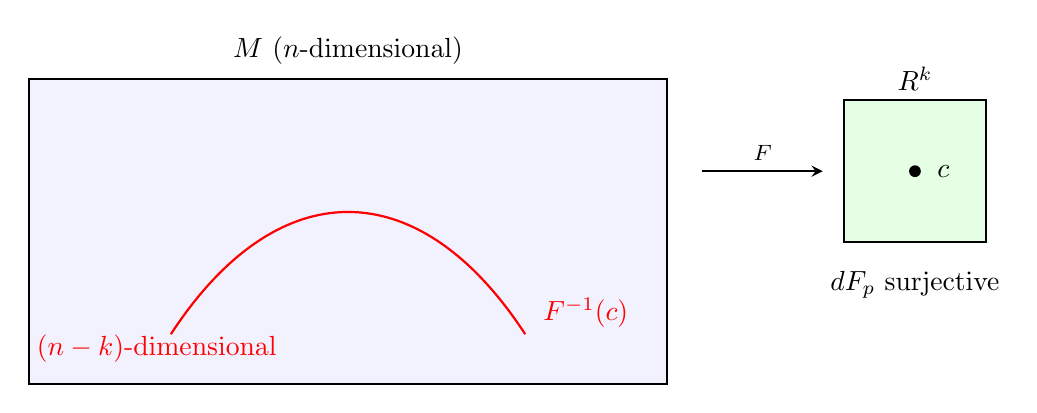
\begin{tikzpicture}[scale=0.9]

  \node at (0,3.2) {$M$ ($n$-dimensional)};
  \draw[thick, fill=blue!5] (-4.5,-1.5) rectangle (4.5,2.8);

  \draw[thick, red] (-2.5,-0.8) .. controls (-1,1.5) and (1,1.5) .. (2.5,-0.8);
  \node[red, xshift=0.5cm] at (2.8,-0.5) {$F^{-1}(c)$};
  \node[red] at (-2.7,-1.0) {$(n-k)$-dimensional};

  \draw[->, thick, >=stealth] (5.0,1.5) -- node[above, font=\footnotesize]{$F$} (6.7,1.5);

  \draw[thick, fill=green!10] (7.0,0.5) rectangle (9.0,2.5);
  \node at (8.0,2.8) {$\mathbb{R}^k$};
  \node[circle, fill, inner sep=1.5pt] at (8.0,1.5) {};
  \node at (8.4,1.5) {$c$};
  \node at (8.0,-0.1) {$dF_p$ surjective};
\end{tikzpicture}
\caption{The regular level set theorem: if $dF_p$ is surjective everywhere, then $F^{-1}(c)$ is an embedded submanifold of codimension $k$.}
\label{fig:regular_level_set}
\end{figure}

\begin{corollary}[Level Sets of Conserved Quantities]\label{cor:conservation_levelset}
Let $Q_1, \dots, Q_k$ be independent conserved quantities. Then $\mathcal{M}_{c_1, \dots, c_k} := \{Q_1 = c_1, \dots, Q_k = c_k\}$ is an $(n-k)$-dimensional embedded submanifold.
\end{corollary}

\begin{proof}
Take $F = (Q_1, \dots, Q_k)$; the result follows directly from Theorem \ref{thm:regular_level_set}.
\end{proof}

\section{Riemannian Manifolds}

\begin{definition}[Riemannian Metric]\label{def:riemannian_metric}
Let $M$ be a smooth manifold. A \textbf{Riemannian metric} $g$ on $M$ assigns to each $p \in M$ a positive-definite inner product $g_p: T_pM \times T_pM \to \mathbb{R}$ on the tangent space $T_pM$, and $g$ depends smoothly on $p$. A manifold $(M, g)$ equipped with a Riemannian metric is called a \textbf{Riemannian manifold}.
\end{definition}

\begin{property}[Basic Properties of the Riemannian Metric]\label{prop:riemannian_metric_properties}
Let $(M, g)$ be a Riemannian manifold, $p \in M$, $u, v, w \in T_pM$ and $a, b \in \mathbb{R}$. Then:
\begin{enumerate}[label=(\roman*)]
    \item \textbf{Symmetry}: $g_p(u, v) = g_p(v, u)$;
    \item \textbf{Bilinearity}: $g_p(au + bv, w) = a g_p(u, w) + b g_p(v, w)$;
    \item \textbf{Positive definiteness}: $g_p(v, v) \ge 0$, and $g_p(v, v) = 0 \iff v = 0$;
    \item \textbf{Coordinate representation}: in local coordinates $(x^1, \dots, x^n)$, $g_p(u, v) = \sum_{i,j} g_{ij}(p) u^i v^j$, where $g_{ij}(p) = g_p(\frac{\partial}{\partial x^i}, \frac{\partial}{\partial x^j})$.
\end{enumerate}
\end{property}

\begin{proof}
(i)--(iii) follow directly from the definition of an inner product. (iv) is obtained by expanding $u = \sum_i u^i \frac{\partial}{\partial x^i}$ and $v = \sum_j v^j \frac{\partial}{\partial x^j}$ using bilinearity.
\end{proof}

\begin{proposition}[Norm and Distance Induced by the Riemannian Metric]\label{prop:metric_norm}
The Riemannian metric $g$ induces a norm $\|v\|_p := \sqrt{g_p(v,v)}$ on each tangent space. The length of a curve $\gamma: [a,b] \to M$ is
\[
L(\gamma) = \int_a^b \|\dot{\gamma}(t)\|_{\gamma(t)}\, dt.
\]
The \textbf{Riemannian distance} between two points $p, q$ of $M$ is
\[
d(p,q) = \inf\{L(\gamma) : \gamma \text{ is a piecewise smooth curve joining } p, q\}.
\]
\end{proposition}

\begin{proof}
\textbf{Norm axioms}: (i) Positive definiteness: $\|v\|_p \ge 0$ follows from $g_p(v,v) \ge 0$; $\|v\|_p = 0 \iff g_p(v,v) = 0 \iff v = 0$. (ii) Homogeneity: $\|av\|_p = \sqrt{g_p(av,av)} = \sqrt{a^2 g_p(v,v)} = |a|\|v\|_p$. (iii) Triangle inequality: by the Cauchy--Schwarz inequality $|g_p(u,v)| \le \|u\|_p \|v\|_p$,
\[
\|u+v\|_p^2 = \|u\|_p^2 + 2g_p(u,v) + \|v\|_p^2 \le (\|u\|_p + \|v\|_p)^2.
\]

\textbf{Riemannian distance}: (i) Non-negativity: arc length is non-negative, hence $d(p,q)\ge0$. (ii) Symmetry: reversing the curve gives $d(p,q) = d(q,p)$. (iii) Triangle inequality: concatenating a curve from $p$ to $q$ with a curve from $q$ to $r$ gives $d(p,r) \le d(p,q) + d(q,r)$. (iv) Positive definiteness: $d(p,p) = 0$ (take a constant curve). If $p \neq q$, then in local coordinates $g_{ij}$ is positive definite, so there exists a constant $c > 0$ with $\|v\| \ge c |v|_{\text{Euclidean}}$; hence every curve joining $p, q$ has length at least $c \cdot |\varphi(p) - \varphi(q)| > 0$, and $d(p,q) > 0$.
\end{proof}

\begin{definition}[Gradient Under the Riemannian Metric]\label{def:riemannian_gradient}
Let $(M, g)$ be a Riemannian manifold and $f \in C^\infty(M)$. The \textbf{gradient} $\nabla f$ of $f$ is the vector field on $M$ defined by:
\[
g_p(\nabla f(p), v) = df_p(v), \qquad \forall v \in T_pM.
\]
\end{definition}

\begin{proposition}[Orthogonality of the Gradient and the Level Set]\label{prop:gradient_orthogonal_levelset}
Let $(M,g)$ be a Riemannian manifold, $f \in C^\infty(M)$ and $c \in \mathbb{R}$. If $p \in f^{-1}(c)$ and $\nabla f(p) \neq 0$, then $\nabla f(p)$ is orthogonal to the tangent space of the level set $f^{-1}(c)$ at $p$.
\end{proposition}

\begin{figure}[htbp]
\centering
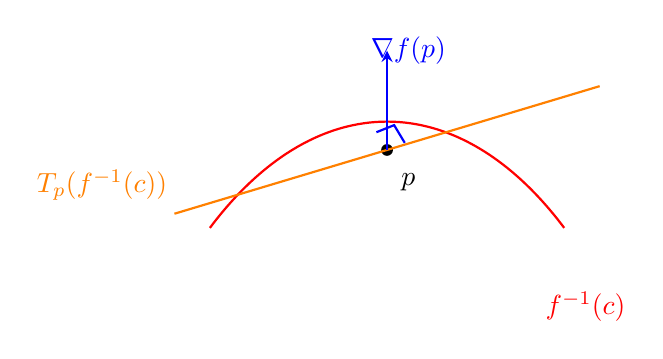
\begin{tikzpicture}[scale=0.9]

  \draw[thick, red] (-2.5,-0.5) .. controls (-1,1.5) and (1,1.5) .. (2.5,-0.5);
  \node[red, yshift=-1cm] at (2.8,-0.5) {$f^{-1}(c)$};

  \node[circle, fill, inner sep=1.5pt] (p) at (0,0.6) {};
  \node[yshift=-0.5cm] at (0.3,0.7) {$p$};

  \draw[thick, orange] (-3,-0.3) -- (3,1.5);
  \node[orange, xshift=-2cm] at (-1.8,0.1) {$T_p(f^{-1}(c))$};

  \draw[->, thick, blue, >=stealth] (0,0.6) -- (0.0,2.0);
  \node[blue] at (0.3,2.0) {$\nabla f(p)$};

  \draw[thick, blue] (-0.15,0.85) -- (0.1,0.95) -- (0.25,0.7);
\end{tikzpicture}
\caption{The gradient is orthogonal to the level set: $\nabla f(p)$ is perpendicular to the tangent space of the level set at $p$.}
\label{fig:gradient_levelset}
\end{figure}

\begin{proof}
Let $v \in T_p(f^{-1}(c))$. Take a curve $\gamma: (-\varepsilon, \varepsilon) \to f^{-1}(c)$ with $\gamma(0) = p$ and $\dot{\gamma}(0) = v$. Then $f(\gamma(t)) = c$ for all $t$, hence
\[
0 = \left. \frac{d}{dt} \right|_{t=0} f(\gamma(t)) = df_p(v) = g_p(\nabla f(p), v).
\]
Therefore $\nabla f(p)$ is orthogonal to $T_p(f^{-1}(c))$.
\end{proof}

\begin{remark}[The Role of the Riemannian Metric]\label{rem:riemannian_central}
The Riemannian metric serves two functions in this chapter. First, it is the basis for the definition of the \textbf{normal space} (Definition \ref{def:normal_space}) --- the normal space is defined by means of the orthogonal complement. Second, it is the basis for the definition of the \textbf{energy norm} $\|\dot{\gamma}\|^2$ of a curve, and thereby supplies the metric structure for the variational principle (the geodesic equation) and for symplectic geometry (the phase-space volume form).
\end{remark}

\section{Fibre Bundles}

\begin{definition}[Fibre Bundle]\label{def:fibre_bundle}
Let $E, B, F$ be smooth manifolds and $\pi: E \to B$ a smooth surjection. The quadruple $(E, B, \pi, F)$ is called a \textbf{fibre bundle} if it satisfies the \textbf{local trivialisation condition}: for every $b \in B$ there exist an open neighbourhood $U \ni b$ and a diffeomorphism $\Phi: \pi^{-1}(U) \to U \times F$ such that $\pi = \text{pr}_1 \circ \Phi$.
\end{definition}

\begin{figure}[htbp]
\centering
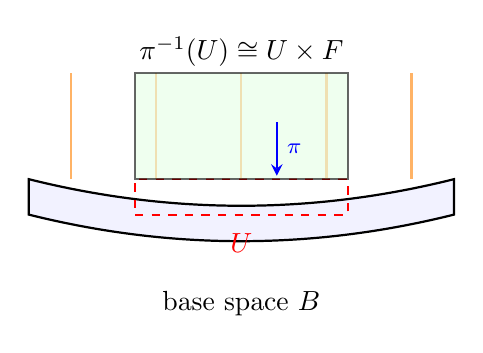
\begin{tikzpicture}[scale=0.9]

  \draw[thick, fill=blue!5] (-3,-0.5) .. controls (-1,-1.0) and (1,-1.0) .. (3,-0.5) -- (3,0) .. controls (1,-0.5) and (-1,-0.5) .. (-3,0) -- cycle;
  \node[yshift=-0.5cm] at (0,-1.2) {base space $B$};

  \draw[thick, dashed, red] (-1.5,-0.5) -- (1.5,-0.5) -- (1.5,0) -- (-1.5,0) -- cycle;
  \node[red] at (0,-0.9) {$U$};

  \foreach \x in {-2.4,-1.2,0,1.2,2.4} {
    \draw[thick, orange, opacity=0.6] (\x,0) -- (\x,1.5);
  }

  \draw[thick, fill=green!10, opacity=0.6] (-1.5,0) rectangle (1.5,1.5);
  \node at (0,1.8) {$\pi^{-1}(U)\cong U\times F$};

  \draw[->, thick, >=stealth, blue] (0.5,0.8) -- node[right, font=\footnotesize]{$\pi$} (0.5,0.05);
\end{tikzpicture}
\caption{Local trivialisation of a fibre bundle: locally $\pi^{-1}(U)\cong U\times F$, and the projection $\pi$ maps $(b,f)$ back to the base point $b$.}
\label{fig:fibre_bundle}
\end{figure}

\begin{definition}[Section of a Fibre Bundle]\label{def:fibre_bundle_section}
A section is a smooth map $s: B \to E$ satisfying $\pi \circ s = \text{id}_B$. The set of all sections is denoted $\Gamma(E)$.
\end{definition}

\begin{proposition}[Tangent and Cotangent Bundles Are Fibre Bundles]\label{prop:tangent_cotangent_bundles}
The tangent bundle $TM$ and the cotangent bundle $T^*M$ are both fibre bundles over $M$, with fibres $\mathbb{R}^n$ and $(\mathbb{R}^n)^*$ respectively.
\end{proposition}

\begin{proof}
This follows directly from the local trivialisation in Proposition \ref{prop:tangent_bundle_manifold}.
The local trivialisation of the cotangent bundle is analogous:
\[
\tilde{\varphi}^*(p, \omega)
= (x^1, \dots, x^n, \omega_1, \dots, \omega_n),
\]
where $\omega = \sum_i \omega_i dx^i$.
\end{proof}

\begin{definition}[Trivial Bundle]\label{def:trivial_bundle}
If there exists a global diffeomorphism $\Phi: E \to B \times F$ with $\pi = \text{pr}_1 \circ \Phi$, then the fibre bundle is called a \textbf{trivial bundle}.
\end{definition}

\begin{definition}[Vector Bundle]\label{def:vector_bundle}
If the fibre $F$ is a vector space and the restriction of each local trivialisation to each fibre is a linear isomorphism, then the fibre bundle is called a \textbf{vector bundle}.
\end{definition}

\begin{property}[Basic Properties of Fibre Bundles]\label{prop:fibre_bundle_properties}
Let $(E, B, \pi, F)$ be a fibre bundle. Then:
\begin{enumerate}[label=(\roman*)]
    \item \textbf{Diffeomorphism type of the fibres}: for any $b_1, b_2$ in the same connected component of $B$, $E_{b_1} \cong E_{b_2} \cong F$;
    \item \textbf{The projection is a submersion}: $\pi$ is a smooth submersion ($d\pi$ is surjective everywhere);
    \item \textbf{Local existence of sections}: for every $b \in B$ there exist an open neighbourhood $U \ni b$ and a local section $s: U \to E$;
    \item \textbf{Module structure of the section space}: if $E$ is a vector bundle, then $\Gamma(E)$ is a $C^\infty(B)$-module.
\end{enumerate}
\end{property}

\begin{proof}
(i) By local trivialisation, $E_b \cong \{b\} \times F \cong F$ holds locally in $b$; the global conclusion on a connected component follows from the transitivity of local properties.
(ii) In a local trivialisation, $d\pi$ corresponds to the differential of the projection $\text{pr}_1: U \times F \to U$, which is surjective.
(iii) In a local trivialisation, take $s(b) = \Phi^{-1}(b, f_0)$ with $f_0 \in F$ fixed.
(iv) Pointwise addition and scalar multiplication of sections give $\Gamma(E)$ its $C^\infty(B)$-module structure.
\end{proof}

\begin{example}[Trivial and Non-Trivial Bundles]\label{ex:trivial_nontrivial_bundle}
\begin{enumerate}[label=(\roman*)]
    \item $T\mathbb{R}^n \cong \mathbb{R}^n \times \mathbb{R}^n$ is a trivial bundle.
    \item $TS^1 \cong S^1 \times \mathbb{R}$ is a trivial bundle (a cylinder).
    \item $TS^2$ is not a trivial bundle (the hairy ball theorem).
\end{enumerate}
\end{example}

\begin{figure}[htbp]
\centering
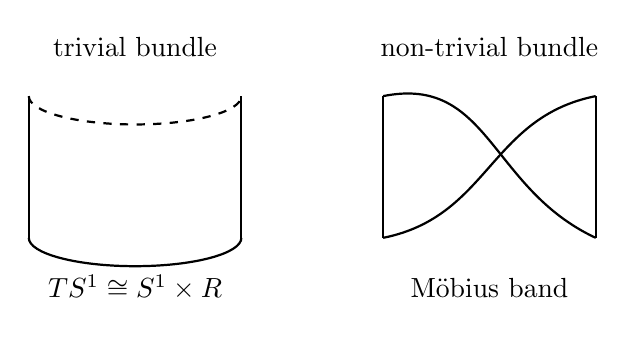
\begin{tikzpicture}[scale=0.9]

  \draw[thick] (-1.5,-1) -- (-1.5,1);
  \draw[thick] (1.5,-1) -- (1.5,1);
  \draw[thick] (-1.5,-1) arc (180:360:1.5 and 0.4);
  \draw[thick, dashed] (-1.5,1) arc (180:360:1.5 and 0.4);
  \node at (0,-1.7) {$TS^1\cong S^1\times\mathbb R$};
  \node at (0,1.7) {trivial bundle};

  \begin{scope}[shift={(5,0)}]
    \draw[thick] (-1.5,-1) .. controls (0,-0.7) and (0,0.7) .. (1.5,1);
    \draw[thick] (-1.5,1) .. controls (0,1.3) and (0,-0.3) .. (1.5,-1);
    \draw[thick] (-1.5,-1) -- (-1.5,1);
    \draw[thick] (1.5,-1) -- (1.5,1);
    \node at (0,-1.7) {M\"obius band};
    \node at (0,1.7) {non-trivial bundle};
  \end{scope}
\end{tikzpicture}
\caption{Comparison of a trivial bundle (a cylinder) with a non-trivial bundle (the M\"obius band).}
\label{fig:trivial_nontrivial}
\end{figure}

\section{Normal Space and Normal Bundle}

\begin{definition}[Normal Space]\label{def:normal_space}
Let $(M, g)$ be a Riemannian manifold, $S \subseteq M$ an embedded submanifold and $p \in S$. The \textbf{normal space} of $S$ at $p$ is $N_pS := \{v \in T_pM : g_p(v, w) = 0, \forall w \in T_pS\}$.
\end{definition}

\begin{definition}[Normal Bundle]\label{def:normal_bundle}
The \textbf{normal bundle} of $S$ is $NS := \bigsqcup_{p \in S} N_pS$.
\end{definition}

\begin{figure}[htbp]
\centering
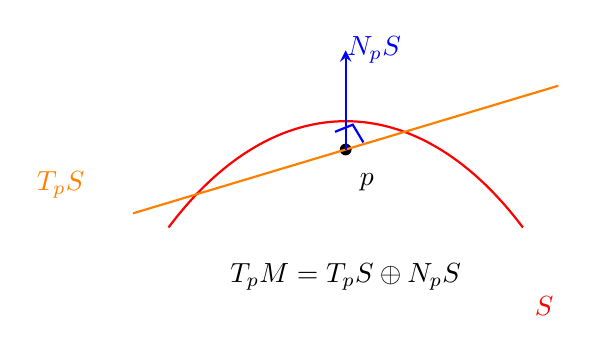
\begin{tikzpicture}[scale=0.9]

  \draw[thick, red] (-2.5,-0.5) .. controls (-1,1.5) and (1,1.5) .. (2.5,-0.5);
  \node[red, yshift=-1cm] at (2.8,-0.5) {$S$};

  \node[circle, fill, inner sep=1.5pt] (p) at (0,0.6) {};
  \node[yshift=-0.5cm] at (0.3,0.7) {$p$};

  \draw[thick, orange] (-3,-0.3) -- (3,1.5);
  \node[orange, xshift=-2cm] at (-1.8,0.1) {$T_pS$};

  \draw[thick, blue, ->, >=stealth] (0,0.6) -- (0,2.0);
  \node[blue] at (0.4,2.0) {$N_pS$};

  \draw[thick, blue] (-0.15,0.85) -- (0.1,0.95) -- (0.25,0.7);

  \node at (0,-1.2) {$T_pM=T_pS\oplus N_pS$};
\end{tikzpicture}
\caption{The normal space $N_pS$ is the orthogonal complement of the tangent space $T_pS$ in $T_pM$, $T_pM=T_pS\oplus N_pS$.}
\label{fig:normal_space}
\end{figure}

\begin{proposition}[Gradient of Conserved Quantity and Normal Space]\label{prop:normal_bundle_constraint}
Let $Q_1, \dots, Q_k$ be independent conserved quantities and $\mathcal{M}$ the level-set submanifold. Then $N_p\mathcal{M} = \operatorname{span}\{\nabla Q_1(p), \dots, \nabla Q_k(p)\}$.
\end{proposition}

\begin{proof}
By Proposition \ref{prop:gradient_orthogonal_levelset}, $\nabla Q_i(p) \in N_p\mathcal{M}$. By independence they are linearly independent and span a $k$-dimensional space, which is exactly the dimension of the normal space.
\end{proof}

\section{Angle Space and Angle Bundle}

\begin{definition}[Angle Space]\label{def:angle_space}
Let $\gamma: [0, T] \to M$ be a closed orbit. The \textbf{angle space} $A_\gamma$ on $\gamma$ is the parametrisation space of the orbit itself: when $\gamma$ is a contractible closed curve, one takes $A_\gamma \cong U(1)$; when $\gamma$ has a fundamental group element of finite order, one takes $A_\gamma \cong \mathbb{Z}_T$.
\end{definition}

\begin{definition}[Angle Bundle]\label{def:angle_bundle}
The \textbf{angle bundle} $AM := \bigsqcup_{\alpha} A_{\gamma_\alpha}$ is the union of the angle spaces over the family of closed orbits.
\end{definition}

\begin{proposition}[Algebraic Structure of the Angle Space]\label{prop:angle_space_topology}
The topological structure of the angle space determines the type of the natural group structure on it: the continuous circle $U(1)$ corresponds to a continuous rotation group, and the finite cyclic group $\mathbb{Z}_T$ corresponds to a finite rotation group.
\end{proposition}

\begin{figure}[htbp]
\centering
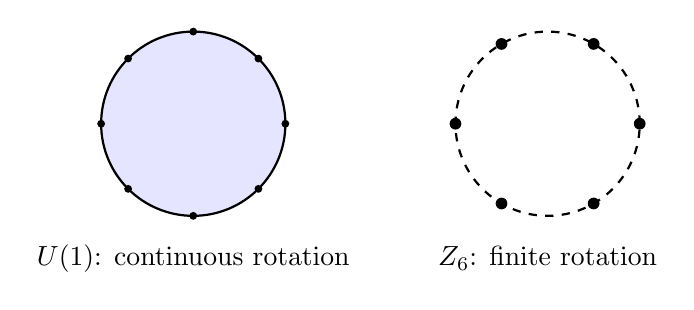
\begin{tikzpicture}[scale=0.9]

  \draw[thick, fill=blue!10] (0,0) circle (1.3);
  \foreach \a in {0,45,90,135,180,225,270,315} {
    \node[circle, fill, inner sep=1pt] at (\a:1.3) {};
  }
  \node at (0,-1.9) {$U(1)$: continuous rotation};

  \begin{scope}[shift={(5,0)}]
    \draw[thick, dashed] (0,0) circle (1.3);
    \foreach \a in {0,60,120,180,240,300} {
      \node[circle, fill, inner sep=1.5pt] at (\a:1.3) {};
    }
    \node at (0,-1.9) {$\mathbb{Z}_6$: finite rotation};
  \end{scope}
\end{tikzpicture}
\caption{The two topological types of angle space: the continuous circle $U(1)$ and the finite cyclic group $\mathbb{Z}_T$.}
\label{fig:angle_space}
\end{figure}

\begin{proof}
\textbf{Continuous case}: $U(1) = \{e^{i\theta} : \theta \in [0, 2\pi)\}$. Let us verify that $U(1)$ is a group: (i) Closure: $e^{i\theta}e^{i\phi} = e^{i(\theta+\phi)} \in U(1)$; (ii) associativity follows from the associativity of complex multiplication; (iii) the identity element is $e^{i0} = 1$; (iv) the inverse is $(e^{i\theta})^{-1} = e^{-i\theta} \in U(1)$. $U(1)$ is a compact connected one-dimensional Lie group.

\textbf{Discrete case}: $\mathbb{Z}_T = \{0, 1, \dots, T-1\}$ is the cyclic group $C_T$ under addition modulo $T$. The map $k \mapsto e^{i2\pi k/T}$ gives an injective group homomorphism $C_T \to U(1)$, whose image is the group of $T$-th roots of unity.
\end{proof}

\section{Phase Space}

\begin{definition}[Configuration Space]\label{def:configuration_space}
Let the position of a mechanical system be described by $n$ generalised coordinates. The set $Q$ of all possible positions is an $n$-dimensional smooth manifold, called the \textbf{configuration space}.
\end{definition}

\begin{definition}[State-Space Manifold]\label{def:state_space_manifold}
The \textbf{state-space manifold} $M$ is the set of all possible states of the system, equipped with a smooth manifold structure. A periodic orbit is a closed curve in $M$.
\end{definition}

\begin{definition}[Phase Space---Tangent Bundle Formulation]\label{def:phase_space_tangent}
In Lagrangian mechanics, \textbf{phase space} is $TQ$, with elements $(q, \dot{q})$.
\end{definition}

\begin{definition}[Phase Space---Cotangent Bundle Formulation]\label{def:phase_space_cotangent}
In Hamiltonian mechanics, \textbf{phase space} is $T^*Q$, with elements $(q, p)$. $T^*Q$ carries the symplectic structure $\omega = \sum_i dq^i \wedge dp_i$.
\end{definition}

\begin{figure}[htbp]
\centering
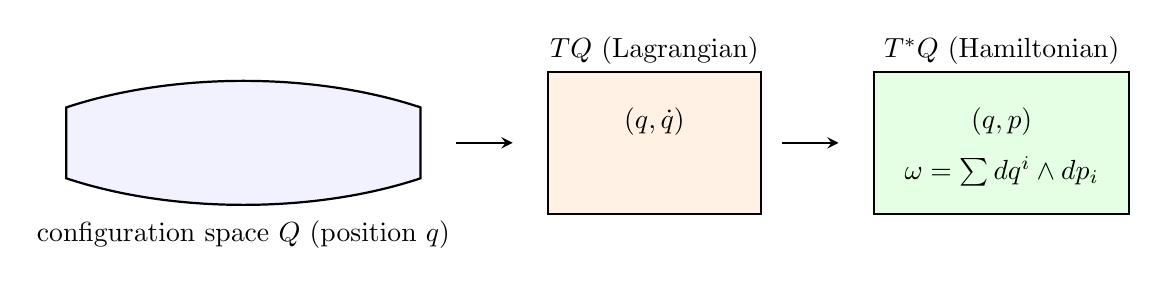
\begin{tikzpicture}[scale=0.9]

  \draw[thick, fill=blue!5] (-2.5,-0.5) .. controls (-1,-1) and (1,-1) .. (2.5,-0.5) -- (2.5,0.5) .. controls (1,1) and (-1,1) .. (-2.5,0.5) -- cycle;
  \node at (0,-1.3) {configuration space $Q$ (position $q$)};

  \draw[->, thick, >=stealth] (3.0,0) -- (3.8,0);
  \draw[thick, fill=orange!10] (4.3,-1) rectangle (7.3,1);
  \node at (5.8,1.3) {$TQ$ (Lagrangian)};
  \node at (5.8,0.3) {$(q,\dot q)$};

  \draw[->, thick, >=stealth] (7.6,0) -- (8.4,0);
  \draw[thick, fill=green!10] (8.9,-1) rectangle (12.5,1);
  \node at (10.7,1.3) {$T^*Q$ (Hamiltonian)};
  \node at (10.7,0.3) {$(q,p)$};
  \node at (10.7,-0.4) {$\omega=\sum dq^i\wedge dp_i$};
\end{tikzpicture}
\caption{The two phase-space formulations, from the configuration space $Q$ to the tangent bundle $TQ$ (Lagrangian) and the cotangent bundle $T^*Q$ (Hamiltonian).}
\label{fig:phase_space}
\end{figure}

\begin{proposition}[Phase-Space Volume and Liouville's Theorem]\label{prop:phase_volume_liouville}
The symplectic volume form on phase space $T^*Q$ is $d\mu = \frac{1}{n!}\omega^n$. The phase-space volume is preserved by the Hamiltonian flow.
\end{proposition}

\begin{proof}
The Hamiltonian vector field $X_H$ in symplectic coordinates $(q^1, \dots, q^n, p_1, \dots, p_n)$ is
\[
X_H = \sum_i \left( \frac{\partial H}{\partial p_i} \frac{\partial}{\partial q^i} - \frac{\partial H}{\partial q^i} \frac{\partial}{\partial p_i} \right).
\]
Its divergence is
\[
\operatorname{div} X_H = \sum_i \left( \frac{\partial}{\partial q^i} \frac{\partial H}{\partial p_i} + \frac{\partial}{\partial p_i} \left( -\frac{\partial H}{\partial q^i} \right) \right) = \sum_i \left( \frac{\partial^2 H}{\partial q^i \partial p_i} - \frac{\partial^2 H}{\partial p_i \partial q^i} \right) = 0,
\]
by Clairaut's theorem the mixed partial derivatives are equal. By Liouville's formula the volume of the flow is preserved.
\end{proof}

\section{Invariant Manifolds and Energy Surfaces}

\begin{definition}[Flow and Invariant Submanifold]\label{def:invariant_submanifold}
Let $X$ be a vector field and $\Phi_t$ its flow. A submanifold $S$ is called an \textbf{invariant submanifold} if $\Phi_t(S) \subseteq S$ for all $t$.
\end{definition}

\begin{proposition}[Level Sets of Conserved Quantities Are Invariant Submanifolds]\label{prop:levelset_invariant}
The level set $Q^{-1}(c)$ of a conserved quantity $Q$ is an invariant submanifold.
\end{proposition}

\begin{proof}
For $p \in Q^{-1}(c)$ we have $Q(p) = c$. By conservation, $Q(\Phi_t(p)) = Q(p) = c$, hence $\Phi_t(p) \in Q^{-1}(c)$.
\end{proof}

\begin{definition}[Energy Surface]\label{def:energy_surface}
Let $H: T^*Q \to \mathbb{R}$ be a Hamiltonian function. The \textbf{energy surface} $\Sigma_E := H^{-1}(E)$ is a constraint hypersurface in phase space.
\end{definition}

\begin{proposition}[Dimension of the Energy Surface]\label{prop:energy_surface_dimension}
If $dH \neq 0$ holds everywhere on $\Sigma_E$, then $\Sigma_E$ is a $(2n-1)$-dimensional embedded submanifold.
\end{proposition}

\begin{proof}
This follows directly from Theorem \ref{thm:regular_level_set}.
\end{proof}

\begin{figure}[htbp]
\centering
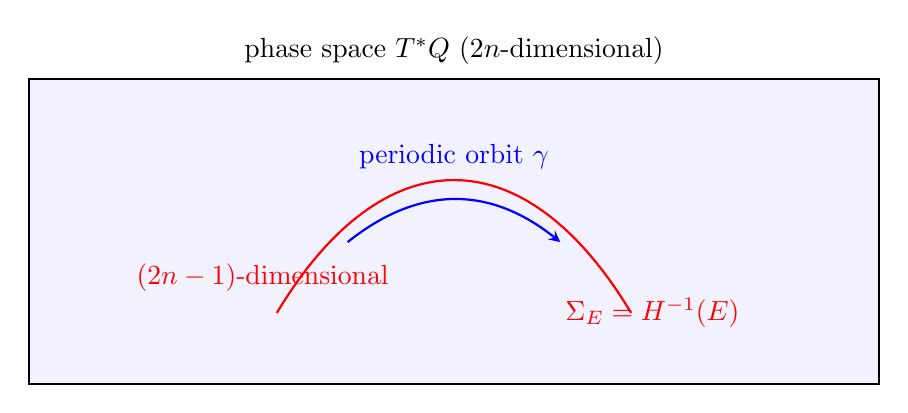
\begin{tikzpicture}[scale=0.9]

  \node at (0,3.2) {phase space $T^*Q$ ($2n$-dimensional)};
  \draw[thick, fill=blue!5] (-6,-1.5) rectangle (6,2.8);

  \draw[thick, red] (-2.5,-0.5) .. controls (-1,2.0) and (1,2.0) .. (2.5,-0.5);
  \node[red] at (2.8,-0.5) {$\Sigma_E=H^{-1}(E)$};
  \node[red] at (-2.7,0.0) {$(2n-1)$-dimensional};

  \draw[thick, blue, ->, >=stealth] (-1.5,0.5) .. controls (-0.5,1.3) and (0.5,1.3) .. (1.5,0.5);
  \node[blue] at (0,1.7) {periodic orbit $\gamma$};
\end{tikzpicture}
\caption{The energy surface $\Sigma_E$ is a $(2n-1)$-dimensional hypersurface in phase space, on which periodic orbits move.}
\label{fig:energy_surface}
\end{figure}

\section{Invariant Tori and the Liouville--Arnold Theorem}
\label{sec:invariant_torus}

\begin{definition}[Invariant Torus]\label{def:invariant_torus}
Let a Hamiltonian system have $n$ independent first integrals in involution $F_1 = H, F_2, \dots, F_n$. The level set $\mathbb{T}_{c_1, \dots, c_n} := \{F_1 = c_1, \dots, F_n = c_n\}$ is called an \textbf{invariant torus}.
\end{definition}

\begin{proposition}[Motion on the Invariant Torus]\label{prop:invariant_torus_motion}
On the invariant torus $\mathbb{T}^n$ the motion is described by the angle coordinates $(\theta_1, \dots, \theta_n)$ and satisfies $\dot{\theta}_i = \omega_i$ (constants). Hence $\theta_i(t) = \theta_i(0) + \omega_i t$.
\end{proposition}

\begin{figure}[htbp]
\centering
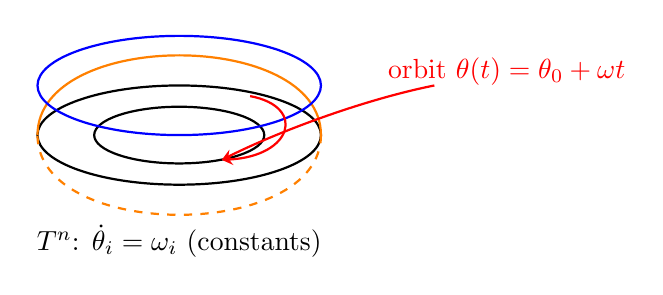
\begin{tikzpicture}[scale=0.9]

  \draw[thick] (0,0) ellipse (2.0 and 0.7);
  \draw[thick] (0,0) ellipse (1.2 and 0.4);

  \draw[thick, orange] (2.0,0) .. controls (2.0,1.5) and (-2.0,1.5) .. (-2.0,0);
  \draw[thick, orange, dashed] (2.0,0) .. controls (2.0,-1.5) and (-2.0,-1.5) .. (-2.0,0);

  \draw[thick, blue] (0,0.7) ellipse (2.0 and 0.7);

  \draw[thick, red, ->, >=stealth]
       (1.0,0.55) .. controls (1.8,0.4) and (1.6,-0.3) .. (0.6,-0.35) coordinate (redtip);

  \node[red, xshift=2cm] at (2.4,0.9) {orbit $\theta(t)=\theta_0+\omega t$};

  \draw[->, thick, red, >=stealth]
       (3.6,0.7) .. controls (2.6,0.5) and (1.4,0.05) .. (redtip);

  \node at (0,-1.5) {$\mathbb{T}^n$: $\dot\theta_i=\omega_i$ (constants)};
\end{tikzpicture}
\caption{Uniform motion on an invariant torus: the angle coordinates evolve according to $\theta_i(t)=\theta_i(0)+\omega_i t$.}
\label{fig:invariant_torus}
\end{figure}

\begin{proof}
This is a direct corollary of Theorem \ref{thm:liouville_arnold}: in action-angle coordinates, $\dot{\theta}_i = \frac{\partial H}{\partial I_i} = \omega_i(I)$ (constants) and $\dot{I}_i = 0$.
\end{proof}

\begin{theorem}[Liouville--Arnold Theorem]\label{thm:liouville_arnold}
Let an $n$-degree-of-freedom Hamiltonian system have $n$ independent first integrals in involution, and suppose that the level set is compact and connected. Then this level set is diffeomorphic to $\mathbb{T}^n$, and near it there exist action-angle coordinates in which the motion becomes uniform rectilinear motion.
\end{theorem}

\begin{proof}
\textbf{The proof lies beyond the scope of this book} (see Arnold, \textit{Mathematical Methods of Classical Mechanics}, 2nd ed., Springer, 1989, \S{}49--50). The core idea: $n$ first integrals in involution generate $n$ commuting flows, and the action of these flows on the level set gives the torus structure.
\end{proof}

\begin{corollary}[Criterion for Closed and Quasi-Periodic Orbits]\label{cor:torus_closure_criterion}
On an invariant torus $\mathbb{T}^n$, an orbit $\theta(t)=\theta_0+\omega t$ is closed if and only if the frequencies are pairwise commensurable, that is, there exists $T>0$ with $\omega T\in2\pi\mathbb{Z}^n$ (equivalently $\omega_i/\omega_j\in\mathbb{Q}$ for all $i,j$); otherwise the orbit is dense in $\mathbb{T}^n$.
\end{corollary}

\begin{proof}
The orbit $\theta(t) = \theta_0 + \omega t$ is closed if and only if there exists $T > 0$ with $\omega T \in 2\pi\mathbb{Z}^n$. This is equivalent to $\omega_i / \omega_j \in \mathbb{Q}$ for all $i,j$ (when $\omega_j \neq 0$). If some $\omega_j=0$, that component is stationary, and it suffices to take $T$ to be the least common multiple of the periods of the remaining components. If the frequencies are pairwise commensurable, take $T$ to be the least common multiple of the periods of the individual frequencies; if there exists a pair of incommensurable frequencies, the orbit is dense in the torus (the Kronecker approximation theorem).
\end{proof}

\begin{figure}[htbp]
\centering
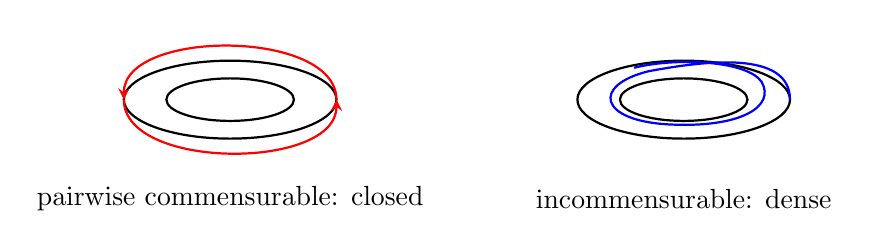
\begin{tikzpicture}[scale=0.9]
  % Left: pairwise commensurable --- a closed orbit
  \begin{scope}[shift={(-3.2,0)}]
    \draw[thick] (0,0) ellipse (1.5 and 0.55);
    \draw[thick] (0,0) ellipse (0.9 and 0.3);
    \draw[thick, red, ->, >=stealth] (1.5,0) .. controls (1.5,1.0) and (-1.5,1.0) .. (-1.5,0);
    \draw[thick, red, ->, >=stealth] (-1.5,0) .. controls (-1.5,-1.0) and (1.5,-1.0) .. (1.5,0);
    \node at (0,-1.4) {pairwise commensurable: closed};
  \end{scope}
  % Right: incommensurable --- a dense orbit
  \begin{scope}[shift={(3.2,0)}]
    \draw[thick] (0,0) ellipse (1.5 and 0.55);
    \draw[thick] (0,0) ellipse (0.9 and 0.3);
    \draw[thick, blue] (1.5,0) .. controls (1.5,0.7) and (0.3,0.55) .. (-0.5,0.4)
                                .. controls (-1.3,0.2) and (-1.2,-0.3) .. (-0.2,-0.35)
                                .. controls (0.8,-0.4) and (1.3,-0.1) .. (1.1,0.25)
                                .. controls (0.9,0.55) and (-0.1,0.6) .. (-0.7,0.45);
    \node at (0,-1.4) {incommensurable: dense};
  \end{scope}
\end{tikzpicture}
\caption{Criterion for the closure of an orbit on an invariant torus: when the frequencies are pairwise commensurable the orbit is closed, and when they are incommensurable the orbit is dense in the torus.}
\label{fig:torus_closure}
\end{figure}

\section{Stable Manifolds, Unstable Manifolds and Centre Manifolds}

\begin{definition}[Stable and Unstable Manifolds]\label{def:stable_unstable_manifold}
Let $\gamma$ be a periodic orbit. $W^s(\gamma) := \{p : d(\Phi_t(p), \gamma) \to 0 \ (t \to +\infty)\}$, $W^u(\gamma) := \{p : d(\Phi_t(p), \gamma) \to 0 \ (t \to -\infty)\}$.
\end{definition}

\begin{definition}[Centre Manifold]\label{def:centre_manifold}
$W^c(\gamma)$ consists of the orbits that neither approach $\gamma$ exponentially nor recede from it exponentially.
\end{definition}

\begin{proposition}[Stable/Unstable Manifolds and Floquet Multipliers]\label{prop:stable_floquet}
Let $\gamma$ be a periodic orbit with Floquet multipliers $\rho_1, \dots, \rho_n$. Then $\dim W^s = \#\{|\rho_i| < 1\}$, $\dim W^u = \#\{|\rho_i| > 1\}$, $\dim W^c = \#\{|\rho_i| = 1\}$.
\end{proposition}

\begin{proof}
By Floquet theory, the linearised dynamics near a periodic orbit is determined by the Floquet multipliers. Write $\rho_i = e^{\lambda_i T}$ ($\lambda_i$ the Floquet exponents). Then $|\rho_i| < 1 \iff \operatorname{Re}\lambda_i < 0$, corresponding to exponential decay (a stable direction); $|\rho_i| > 1 \iff \operatorname{Re}\lambda_i > 0$, corresponding to exponential growth (an unstable direction); $|\rho_i| = 1 \iff \operatorname{Re}\lambda_i = 0$, corresponding to a neutral direction (a centre direction). The dimensions of the stable manifold, the unstable manifold and the centre manifold are equal to the numbers of stable, unstable and centre directions respectively.
\end{proof}

\begin{figure}[htbp]
\centering
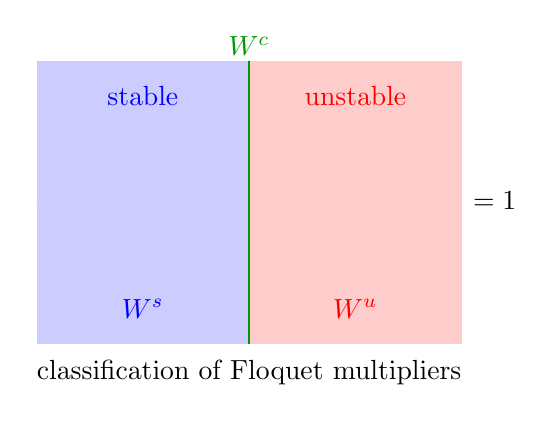
\begin{tikzpicture}[scale=0.9]
  % Coordinate axes
  \draw[->, thick, >=stealth] (-3,0) -- (3,0);
  \draw[->, thick, >=stealth] (0,-2) -- (0,2);
  \node at (3.2,0) {$|\rho|=1$};
  % Stable region
  \fill[blue!20] (-3,0) rectangle (0,2);
  \fill[blue!20] (-3,-2) rectangle (0,0);
  \node[blue] at (-1.5,1.5) {stable};
  \node[blue] at (-1.5,-1.5) {$W^s$};
  % Unstable region
  \fill[red!20] (0,0) rectangle (3,2);
  \fill[red!20] (0,-2) rectangle (3,0);
  \node[red] at (1.5,1.5) {unstable};
  \node[red] at (1.5,-1.5) {$W^u$};
  % Centre axis
  \draw[thick, green!60!black] (0,-2) -- (0,2);
  \node[green!60!black] at (0,2.2) {$W^c$};
  \node at (0,-2.4) {classification of Floquet multipliers};
\end{tikzpicture}
\caption{The stable manifold $W^s$, the unstable manifold $W^u$ and the centre manifold $W^c$ classified by the modulus of the Floquet multipliers.}
\label{fig:stable_manifolds}
\end{figure}

\section{Moduli Space}

\begin{definition}[Moduli Space]\label{def:moduli_space}
Let $\mathcal{S}$ be a collection of periodic structures of a certain kind and $\sim$ an equivalence relation. The \textbf{moduli space} $\mathcal{M} := \mathcal{S}/\sim$ is the set of equivalence classes.
\end{definition}

\begin{example}[Moduli Space of a Periodic Lattice]\label{ex:lattice_moduli_space}
The moduli space of the two-dimensional periodic lattice $\Lambda = \omega_1\mathbb{Z} + \omega_2\mathbb{Z}$ is $SL(2,\mathbb{Z}) \setminus \mathbb{H}$, where $\mathbb{H} = \{\tau \in \mathbb{C} : \operatorname{Im}\tau > 0\}$.
\end{example}

\begin{remark}[Role of the Moduli Space]\label{rem:moduli_space_role}
The moduli space provides a \textbf{classifying space} for periodic structures: periodic structures with the same basic structure are parametrised by the same point of the moduli space, and their deformations are described by the tangent space of the moduli space.
\end{remark}

\begin{figure}[htbp]
\centering
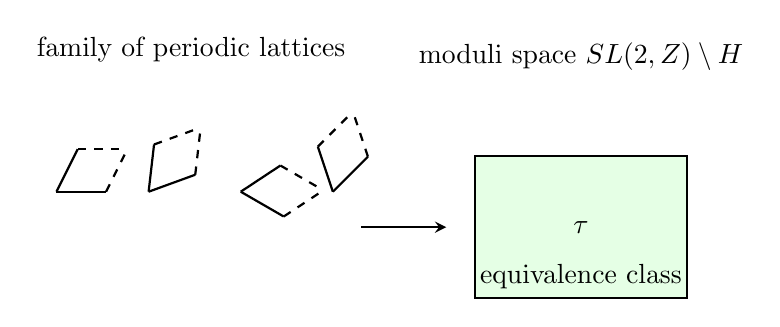
\begin{tikzpicture}[scale=0.9, yshift=-1cm]

  \foreach \x/\y/\ang in {-3.5/1.0/0, -2.2/1.0/20, -0.9/1.0/-30, 0.4/1.0/45} {
    \begin{scope}[shift={(\x,\y)}, rotate=\ang]
      \draw[thick] (0,0) -- (0.7,0);
      \draw[thick] (0,0) -- (0.3,0.6);
      \draw[thick, dashed] (0.7,0) -- (1.0,0.6);
      \draw[thick, dashed] (0.3,0.6) -- (1.0,0.6);
    \end{scope}
  }

  \node[yshift=1cm] at (-1.6,1.9) {family of periodic lattices};

  \draw[->, thick, >=stealth] (0.8,0.5) -- (2.0,0.5);

  \draw[thick, fill=green!10] (2.4,-0.5) rectangle (5.4,1.5);

  \node[yshift=1cm] at (3.9,1.8) {moduli space $SL(2,\mathbb Z)\setminus\mathbb H$};
  \node at (3.9,0.5) {$\tau$};
  \node at (3.9,-0.2) {equivalence class};
\end{tikzpicture}
\caption{The moduli space as a classifying space for periodic structures: equivalence classes are parametrised by $\tau$.}
\label{fig:moduli_space}
\end{figure}

\section{Group Actions and Quotient Manifolds}

\begin{definition}[Action of a Lie Group on a Manifold]\label{def:group_action_manifold}
Let $G$ be a Lie group and $M$ a smooth manifold. A \textbf{smooth left action} of $G$ is a smooth map $\Phi: G \times M \to M$ satisfying $e \cdot p = p$ and $(gh) \cdot p = g \cdot (h \cdot p)$.
\end{definition}

\begin{definition}[Orbits and Quotient Manifolds]\label{def:quotient_manifold}
If the action of $G$ is free and properly discontinuous, then the orbit space $M/G$ carries a unique smooth structure and is called a \textbf{quotient manifold}.
\end{definition}

\begin{proposition}[The Torus as a Quotient Manifold]\label{prop:torus_quotient}
The $n$-dimensional torus is the quotient manifold of Euclidean space by a periodic lattice: $\mathbb{T}^n \cong \mathbb{R}^n / \mathbb{Z}^n$.
\end{proposition}

\begin{figure}[htbp]
\centering
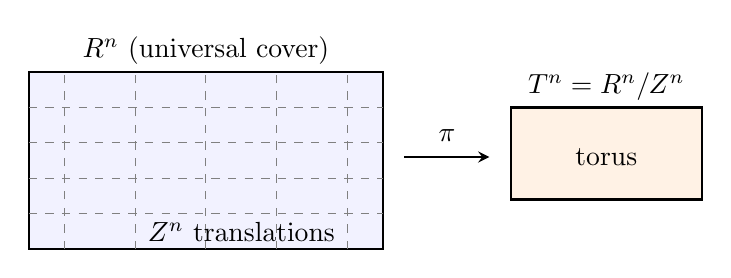
\begin{tikzpicture}[scale=0.9]

  \draw[thick, fill=blue!5] (-2.5,-1) rectangle (2.5,1.5);
  \node at (0,1.8) {$\mathbb{R}^n$ (universal cover)};

  \foreach \x in {-2,-1,0,1,2} {
    \draw[gray, dashed] (\x,-1) -- (\x,1.5);
  }
  \foreach \y in {-0.5,0,0.5,1.0} {
    \draw[gray, dashed] (-2.5,\y) -- (2.5,\y);
  }
  \node at (0.5,-0.75) {$\mathbb{Z}^n$ translations};

  \draw[->, thick, >=stealth] (2.8,0.3) -- (4.0,0.3);
  \node at (3.4,0.6) {$\pi$};
 
  \draw[thick, fill=orange!10] (4.3,-0.3) rectangle (7.0,1.0);
  \node at (5.65,1.3) {$\mathbb{T}^n=\mathbb{R}^n/\mathbb{Z}^n$};
  \node at (5.65,0.3) {torus};
\end{tikzpicture}
\caption{The torus as a quotient manifold: $\mathbb{Z}^n$ acts on $\mathbb{R}^n$ by translations, and taking the quotient yields $\mathbb{T}^n$.}
\label{fig:torus_quotient}
\end{figure}

\begin{proof}
$\mathbb{Z}^n$ acts on $\mathbb{R}^n$ by translations: $(k_1, \dots, k_n) \cdot (x_1, \dots, x_n) = (x_1 + k_1, \dots, x_n + k_n)$.

\textbf{Freeness}: if $(k_1,\dots,k_n)\cdot(x_1,\dots,x_n) = (x_1,\dots,x_n)$, then $x_i + k_i = x_i$, hence $k_i = 0$ for all $i$.

\textbf{Proper discontinuity}: for any compact set $K \subseteq \mathbb{R}^n$ the set $K$ is bounded; let $\|x\| \le R$ for all $x \in K$. If $k \cdot K \cap K \neq \emptyset$, then there exist $x, y \in K$ with $x + k = y$, hence $\|k\| \le 2R$. There are only finitely many integer vectors $(k_1, \dots, k_n)$ satisfying $\|k\| \le 2R$ (each $|k_i| \le 2R$, so at most $(4R+1)^n$ of them). Hence the action is properly discontinuous.

The quotient space $\mathbb{R}^n/\mathbb{Z}^n$ is diffeomorphic to $S^1 \times \cdots \times S^1 = \mathbb{T}^n$ (the diffeomorphism is given by $[(x_1, \dots, x_n)] \mapsto (e^{2\pi i x_1}, \dots, e^{2\pi i x_n})$).
\end{proof}

\begin{definition}[Covering Spaces]\label{def:covering_space}
A surjection $\pi: \tilde{M} \to M$ is called a \textbf{covering map} if for every $p \in M$ there exists an open neighbourhood $U$ such that $\pi^{-1}(U)$ is a union of a family of pairwise disjoint open sets, and $\pi$ maps each of these open sets diffeomorphically onto $U$.
\end{definition}

\begin{lemma}[Basic Properties of Covering Maps]\label{lem:covering_properties}
Let $\pi: \tilde{M} \to M$ be a covering map. Then:
\begin{enumerate}[label=(\roman*)]
    \item \textbf{Local homeomorphism}: $\pi$ is a local diffeomorphism;
    \item \textbf{Discrete fibres}: for every $p \in M$ the fibre $\pi^{-1}(p)$ is a discrete set;
    \item \textbf{Path lifting}: for every $p \in M$, every $\tilde{p} \in \pi^{-1}(p)$ and every path $\gamma: [0,1] \to M$ with $\gamma(0) = p$, there exists a unique lift $\tilde{\gamma}: [0,1] \to \tilde{M}$ satisfying $\tilde{\gamma}(0) = \tilde{p}$ and $\pi \circ \tilde{\gamma} = \gamma$;
    \item \textbf{Homotopy lifting}: homotopic paths lift to homotopic paths.
\end{enumerate}
\end{lemma}

\begin{proof}
(i) follows directly from the definition of a covering map. (ii) follows because $\pi^{-1}(p)$ is a union of disjoint open sets. (iii) Subdivide $[0,1]$ into small subintervals, use the local trivialisation on each subinterval to define the lift, and glue by uniqueness. (iv) This is proved similarly, using the compactness of the homotopy.
\end{proof}

\begin{theorem}[The Real Line Covers the Circle]\label{thm:covering_R_S1}
The map $\pi: \mathbb{R} \to S^1$, $\pi(t) = e^{2\pi i t}$, is a covering map. $\mathbb{R}$ is the universal cover of $S^1$.
\end{theorem}

\begin{figure}[htbp]
\centering
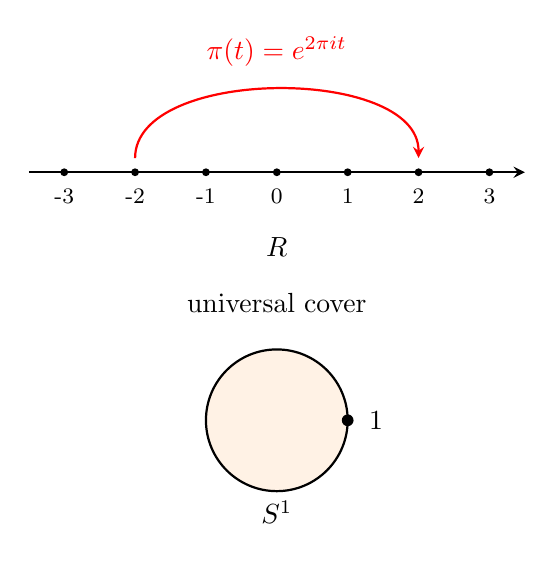
\begin{tikzpicture}[scale=0.9]

  \draw[->, thick, >=stealth] (-3.5,0) -- (3.5,0);
  \foreach \x in {-3,-2,-1,0,1,2,3} {
    \node[circle, fill, inner sep=1pt] at (\x,0) {};
  }
  \node[yshift=-0.5cm] at (0,-0.5) {$\mathbb{R}$};

  \foreach \x in {-3,-2,-1,0,1,2,3} {
    \node[below, font=\footnotesize] at (\x,-0.1) {\x};
  }

  \draw[->, thick, >=stealth, red] (-2,0.2) .. controls (-2,1.5) and (2,1.5) .. (2,0.2);
  \node[red] at (0,1.7) {$\pi(t)=e^{2\pi it}$};

  \draw[thick, fill=orange!10] (0,-3.5) circle (1.0);
  \node[circle, fill, inner sep=1.5pt] at (1.0,-3.5) {};
  \node at (1.4,-3.5) {$1$};
  \node at (0,-4.8) {$S^1$};
  \node[yshift=0.5cm] at (0,-2.4) {universal cover};
\end{tikzpicture}
\caption{The real line $\mathbb{R}$ is the universal cover of the circle $S^1$: $\pi(t)=e^{2\pi i t}$, with fibre $\mathbb{Z}$.}
\label{fig:covering_R_S1}
\end{figure}

\begin{proof}
For any point $e^{i\theta}$ on $S^1$, take the open arc $U = \{e^{i\varphi} : |\varphi - \theta| < \pi\}$. Then $\pi^{-1}(U) = \bigcup_{k \in \mathbb{Z}} (\frac{\theta - \pi}{2\pi} + k, \frac{\theta + \pi}{2\pi} + k)$, and each interval is diffeomorphic to $U$ under $\pi$. $\mathbb{R}$ is simply connected and $\pi$ is a covering, so $\mathbb{R}$ is the universal cover.
\end{proof}

\begin{definition}[Closed Orbits and the Fundamental Group]\label{def:closed_orbit_manifold}
Let $\gamma: [0,T] \to M$ be a closed orbit. Then $\gamma$ defines $[\gamma] \in \pi_1(M)$. If $[\gamma]$ is an element of finite order, then $\gamma$ is called a \textbf{twisted closed orbit}.
\end{definition}

\begin{proposition}[The Fundamental Group of the Torus]\label{prop:periodic_manifold_fundamental_group}
$\pi_1(\mathbb{T}^n) \cong \mathbb{Z}^n$. Closed orbits on the torus are classified by $(k_1, \dots, k_n) \in \mathbb{Z}^n$.
\end{proposition}

\begin{figure}[htbp]
\centering
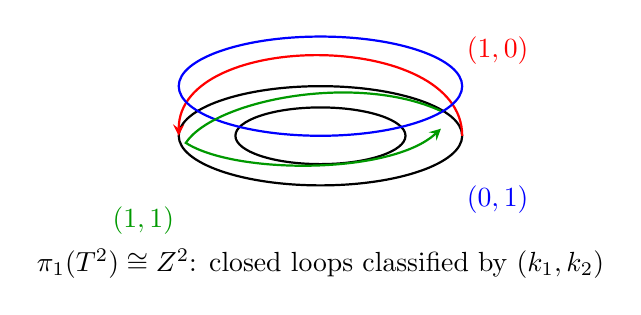
\begin{tikzpicture}[scale=0.9]
  % Schematic of the torus
  \draw[thick] (0,0) ellipse (2.0 and 0.7);
  \draw[thick] (0,0) ellipse (1.2 and 0.4);
  % Meridional closed loop (k1,0)
  \draw[thick, red, ->, >=stealth] (2.0,0) .. controls (2.0,1.5) and (-2.0,1.5) .. (-2.0,0);
  \node[red] at (2.5,1.2) {$(1,0)$};
  % Latitudinal closed loop (0,k2)
  \draw[thick, blue, ->, >=stealth] (0,0.7) ellipse (2.0 and 0.7);
  \node[blue] at (2.5,-0.9) {$(0,1)$};
  % Diagonal closed loop (1,1)
  \draw[thick, green!60!black, ->, >=stealth] (1.7,0.35) .. controls (0.5,0.9) and (-1.5,0.5) .. (-1.9,-0.1)
                                           .. controls (-1.2,-0.55) and (1.0,-0.55) .. (1.7,0.1);
  \node[green!60!black] at (-2.5,-1.2) {$(1,1)$};
  % Explanation
  \node at (0,-1.8) {$\pi_1(\mathbb{T}^2)\cong\mathbb{Z}^2$: closed loops classified by $(k_1,k_2)$};
\end{tikzpicture}
\caption{Closed orbits on the torus are classified by integer vectors in $\pi_1(\mathbb{T}^n)\cong\mathbb{Z}^n$.}
\label{fig:torus_fundamental_group}
\end{figure}

\begin{proof}
By covering theory, $\pi_1(\mathbb{T}^n) \cong \pi_1(S^1)^n$. First we prove that $\pi_1(S^1) \cong \mathbb{Z}$: by Theorem \ref{thm:covering_R_S1}, $\mathbb{R}$ is the universal cover of $S^1$, so $\pi_1(S^1) \cong \pi^{-1}(1) = \mathbb{Z}$ (the group of covering transformations is isomorphic to the fibre). The lift $\tilde{\gamma}$ of a closed curve $\gamma$ on the torus satisfies $\tilde{\gamma}(T) - \tilde{\gamma}(0) = (k_1, \dots, k_n) \in \mathbb{Z}^n$, and this is the element corresponding to $[\gamma]$. Hence $\pi_1(\mathbb{T}^n) \cong \mathbb{Z}^n$.
\end{proof}

\section*{Seven-theme comparison table for this chapter}

\begin{figure}[htbp]
\centering
\begin{tikzpicture}[
  theme/.style={draw, rounded corners, fill=green!10, minimum width=1.2cm, minimum height=0.55cm, align=center, font=\footnotesize}
]
  \node[theme] (p) at (0,0) {Translation};
  \node[theme, right=0.3cm of p] (s) {Scaling};
  \node[theme, right=0.3cm of s] (r) {Rotation};
  \node[theme, right=0.3cm of r] (c) {Conservation};
  \node[theme, right=0.3cm of c] (sym) {Symmetry};
  \node[theme, right=0.3cm of sym] (cl) {Closure};
  \node[theme, right=0.3cm of cl] (per) {Period};
  \node[draw, dashed, rounded corners, fit=(p)(per), inner sep=6pt] (box) {};
  \node[below=0.1cm of box, font=\footnotesize] {the seven themes run through manifolds and fibre bundles};
\end{tikzpicture}
\caption{The seven themes of this chapter: Translation, Scaling, Rotation, Conservation, Symmetry, Closure, Period.}
\label{fig:manifold_themes}
\end{figure}

\begin{center}
\renewcommand{\arraystretch}{1.3}
\begin{tabular}{>{\centering\arraybackslash}p{2.2cm}>{\centering\arraybackslash}p{10.5cm}}
\toprule
Theme & Corresponding content in this chapter \\
\midrule
Translation & the tangent vector as the infinitesimal generator of translation (Definition \ref{def:tangent_vector_derivation}); the orbits of a group action (Definition \ref{def:group_action_manifold}); the covering map (Theorem \ref{thm:covering_R_S1}); uniform motion on an invariant torus (Proposition \ref{prop:invariant_torus_motion}) \\
Scaling & the scaling of the Riemannian metric (Definition \ref{def:riemannian_metric}); the orthogonal complement of the normal space (Definition \ref{def:normal_space}); the parametrisation of the moduli space (Definition \ref{def:moduli_space}) \\
Rotation & the $U(1)$ structure of the angle space (Definition \ref{def:angle_space}); the rotation of the invariant torus (Definition \ref{def:invariant_torus}); stable/unstable manifolds (Definition \ref{def:stable_unstable_manifold}) \\
Conservation & the level set of a conserved quantity (Theorem \ref{thm:regular_level_set}); the energy surface (Definition \ref{def:energy_surface}); the constraints of the normal bundle (Proposition \ref{prop:normal_bundle_constraint}); the invariance of level sets (Proposition \ref{prop:levelset_invariant}) \\
Symmetry & group actions and quotient manifolds (Definition \ref{def:quotient_manifold}); the torus as a quotient manifold (Proposition \ref{prop:torus_quotient}) \\
Closure & closed orbits and the fundamental group (Definition \ref{def:closed_orbit_manifold}); the classification of the fundamental group of the torus (Proposition \ref{prop:periodic_manifold_fundamental_group}); the closure/quasi-periodicity criterion (Corollary \ref{cor:torus_closure_criterion}) \\
Period & the torus as a quotient manifold (Proposition \ref{prop:torus_quotient}); periodic motion on an invariant torus (Proposition \ref{prop:invariant_torus_motion}); the moduli space (Definition \ref{def:moduli_space}) \\
\bottomrule
\end{tabular}
\end{center}

\section*{Exercises}

\begin{enumerate}[leftmargin=3em, label=\textbf{Exercise \arabic*}]
    \item Using Definition \ref{def:topological_manifold}, verify that the circle
    \[
    S^1=\{(x,y)\in\mathbb{R}^2\mid x^2+y^2=1\}
    \]
    is a $1$-dimensional topological manifold. Write down explicitly the two charts
    \[
    U_1=S^1\setminus\{(1,0)\},\quad U_2=S^1\setminus\{(-1,0)\}
    \]
    and the corresponding homeomorphisms $\varphi_1,\varphi_2$, and verify that their union covers $S^1$.

    \item Prove Proposition \ref{prop:tangent_space_basis}:
    let $M$ be an $n$-dimensional smooth manifold, $p\in M$, and let $(U,\varphi=(x^1,\dots,x^n))$ be a chart.
    Then $T_pM$ has dimension $n$, and
    \[
    \left.\frac{\partial}{\partial x^1}\right|_p,\dots,
    \left.\frac{\partial}{\partial x^n}\right|_p
    \]
    forms a basis. Write out the complete proof in the three steps `verifying that it is a tangent vector, linear independence, spanning'.

    \item Verify that the two definitions of a tangent vector are equivalent (Lemma \ref{lem:tangent_vector_equivalence}):
    the derivation definition (Definition \ref{def:tangent_vector_derivation}) and the curve equivalence class definition
    (Definition \ref{def:tangent_vector_curve}) give the same tangent space.
    Write down the correspondence
    \[
    [\gamma]\mapsto v_{[\gamma]},\qquad
    v_{[\gamma]}(f)=\left.\frac{d}{dt}\right|_{t=0}f(\gamma(t)),
    \]
    and prove that it is a well-defined bijection.

    \item Prove the manifold structure of the tangent bundle (Proposition \ref{prop:tangent_bundle_manifold}):
    the tangent bundle $TM$ is a $2n$-dimensional smooth manifold.
    Write down the explicit expression for the local chart $(\pi^{-1}(U),\tilde{\varphi})$
    \[
    \tilde{\varphi}(p,v)=(x^1(p),\dots,x^n(p),v^1,\dots,v^n),
    \]
    and verify the smoothness of the transition map.

    \item Verify Proposition \ref{prop:cotangent_basis}:
    in the chart $(U,\varphi=(x^1,\dots,x^n))$, a basis of the cotangent space $T_p^*M$ is
    \[
    dx^1|_p,\dots,dx^n|_p,
    \]
    satisfying $dx^i|_p(\partial/\partial x^j|_p)=\delta_j^i$.
    Give a proof using the dual basis theorem and the differentials of the coordinate functions.

    \item Prove the regular level set theorem (Theorem \ref{thm:regular_level_set}):
    let $F:M\to\mathbb{R}^k$ be a smooth map and $c\in\mathbb{R}^k$.
    If $dF_p$ is surjective for every $p\in F^{-1}(c)$,
    then $F^{-1}(c)$ is an $(n-k)$-dimensional embedded submanifold.
    Use the rank theorem to construct coordinates near $p$ in which $F=(x^{n-k+1},\dots,x^n)$,
    and write down the local submanifold structure.

    \item Prove Proposition \ref{prop:gradient_orthogonal_levelset}:
    let $(M,g)$ be a Riemannian manifold and $f\in C^\infty(M)$.
    If $p\in f^{-1}(c)$ and $\nabla f(p)\neq0$,
    then $\nabla f(p)$ is orthogonal to the tangent space of the level set $f^{-1}(c)$ at $p$.
    Take a curve $\gamma$ with $f(\gamma(t))=c$ and differentiate with respect to $t$ to complete the proof.

    \item Verify the assertions about trivial and non-trivial bundles in Example \ref{ex:trivial_nontrivial_bundle}:
    \begin{enumerate}[label=(\roman*)]
        \item $T\mathbb{R}^n\cong\mathbb{R}^n\times\mathbb{R}^n$ is a trivial bundle;
        \item $TS^1\cong S^1\times\mathbb{R}$ is a trivial bundle;
        \item $TS^2$ is not a trivial bundle.
    \end{enumerate}
    Use the hairy ball theorem to justify (iii), and explain why there is no continuous tangent vector field on $S^2$ that is nowhere zero.

    \item Prove Proposition \ref{prop:normal_bundle_constraint}:
    let $Q_1,\dots,Q_k$ be independent conserved quantities and $\mathcal{M}$ the level-set submanifold; then
    \[
    N_p\mathcal{M}=\operatorname{span}\{\nabla Q_1(p),\dots,\nabla Q_k(p)\}.
    \]
    Use Proposition \ref{prop:gradient_orthogonal_levelset} to show that $\nabla Q_i(p)\in N_p\mathcal{M}$,
    and use independence to show that they span a $k$-dimensional space.

    \item Prove Proposition \ref{prop:angle_space_topology}:
    the topological structure of the angle space determines the type of the natural group structure on it:
    the continuous circle $U(1)$ corresponds to a continuous rotation group, and the finite cyclic group $\mathbb{Z}_T$ corresponds to a finite rotation group.
    Verify the group axioms for $U(1)$ and $\mathbb{Z}_T$ separately,
    and show that the map $k\mapsto e^{i2\pi k/T}$ gives an injective group homomorphism $C_T\to U(1)$.

    \item Prove, in the Liouville--Arnold theorem (Theorem \ref{thm:liouville_arnold}), the criterion for closed and quasi-periodic orbits (Corollary \ref{cor:torus_closure_criterion}):
    on an invariant torus $\mathbb{T}^n$, an orbit is closed if and only if the frequencies are pairwise commensurable, that is, there exists $T>0$ with $\omega T\in2\pi\mathbb{Z}^n$ (equivalently $\omega_i/\omega_j\in\mathbb{Q}$ for all $i,j$).
    Prove sufficiency and necessity separately, and use the Kronecker approximation theorem to show that the orbit is dense when the frequencies are incommensurable.

    \item Verify Proposition \ref{prop:stable_floquet}:
    let $\gamma$ be a periodic orbit with Floquet multipliers $\rho_1,\dots,\rho_n$. Then
    \[
    \dim W^s=\#\{|\rho_i|<1\},\quad
    \dim W^u=\#\{|\rho_i|>1\},\quad
    \dim W^c=\#\{|\rho_i|=1\}.
    \]
    Complete the proof using the sign of the real part of the Floquet exponents $\lambda_i$.

    \item Prove that the torus is a quotient manifold (Proposition \ref{prop:torus_quotient}):
    the $n$-dimensional torus $\mathbb{T}^n\cong\mathbb{R}^n/\mathbb{Z}^n$.
    Verify that the action of $\mathbb{Z}^n$ on $\mathbb{R}^n$ by translations is free and properly discontinuous,
    and write down the diffeomorphism from the quotient space to $S^1\times\cdots\times S^1$.

    \item Prove that the real line covers the circle (Theorem \ref{thm:covering_R_S1}):
    the map $\pi:\mathbb{R}\to S^1$, $\pi(t)=e^{2\pi it}$, is a covering map,
    and $\mathbb{R}$ is the universal cover of $S^1$.
    Write down an open neighbourhood $U$ of an arbitrary point of $S^1$ and the decomposition of its preimage $\pi^{-1}(U)$,
    and explain why $\mathbb{R}$ is simply connected.

    \item Prove the fundamental group of the torus (Proposition \ref{prop:periodic_manifold_fundamental_group}):
    \[
    \pi_1(\mathbb{T}^n)\cong\mathbb{Z}^n.
    \]
    Use covering space theory to show that $\pi_1(\mathbb{T}^n)\cong\pi_1(S^1)^n$,
    and use the fact that $\mathbb{R}$ is the universal cover of $S^1$ to show that $\pi_1(S^1)\cong\mathbb{Z}$.

    \item Synthesis: combining the tangent space (Definition \ref{def:tangent_vector_derivation}),
    the normal space (Definition \ref{def:normal_space}), the angle space (Definition \ref{def:angle_space})
    and the invariant torus (Definition \ref{def:invariant_torus}),
    explain how the manifold framework answers simultaneously the five questions raised in the introduction:
    whether a group element has finite order, whether an orbit is closed, whether there exists an integrable vector field in the tangential direction,
    whether there exists a conservation constraint in the normal direction, and whether the phase in the angular direction is single-valued.
    Indicate respectively the corresponding theorem or proposition for these structures in this chapter.
\end{enumerate}

